
%%%%%%%%%%%%%%%%%%%%%%%%%%%
% PREAMBOLO DEL DOCUMENTO %
%%%%%%%%%%%%%%%%%%%%%%%%%%%
\documentclass[a4paper,11pt,oneside,top=3cm,bottom=3cm,left=3.5cm,right=3.5cm,openright,reqno,table]{book}

% openany - fa iniziare i capitoli direttamente nella pagina successiva
% openright - fa iniziare i capitoli nella prima pagina destra disponibile 
% fleqn  - allinea le formule a sinistra anzichè centrarle
% leqno - dispone la numerazione delle formule sulla sinistra o destra
% reqno - dispone la numerazione delle formule sulla destra
%
\usepackage{packages}
% Per non appesantire troppo questo file
% quasi tutti i pacchetti usati sono salvati in packages.sty
%
\linespread{1.5}
% Per avere la parola BOZZA scritta su tutte le pagine

% funziona solo in modalità PS
% Invece per i PDF ho risolto così:
% pdftk tesi.pdf background bozza.pdf output tesi_bozza.pdf
%
\newenvironment{nointerlinea}[1]{
\begin{spacing}{#1}}
{\end{spacing}
}
%%%%%%%%%%%%%%%%%%%%%%%%%%%%%%%%%
%   DOCUMENTO VERO E PROPRIO    %
%%%%%%%%%%%%%%%%%%%%%%%%%%%%%%%%%
\begin{document}
% FRONTESPIZIO %
\begin{titlepage}
\changepage{}{}{}{-7.5 mm}{}{}{}{}{}
% parametri per cambiare le dimensioni di una singola pagina in ordine:
% {textheight}{textwidth}{evensidemargin}{oddsidemargin}{columnsep}
% {topmargin}{headheight}{headsep}{footskip}
% se voglio centrare la pagina devo mettere bindingoffset/2
% i primi 5 parametri posso usarli con \changetext


\begin{center}

\includegraphics [width=.15\columnwidth, angle=0]{unisa}\\ % height
\vspace{0.5cm}
{\LARGE \scshape Università degli Studi di Salerno}\\
\vspace{0.5cm}
{\Large Dipartimento di Informatica}\\
\vspace{0.1cm}
{\large Corso di Laurea Magistrale in Informatica}\\
\vspace{1.5cm}
{\Large \scshape Tesi di Laurea} \\
\vspace{4cm}
{\Huge \bfseries TITOLO TESI} \\
\vspace{5cm}

\begin{minipage}[t]{7cm}
\flushleft
\textsc{Relatore}

Prof. \textbf{Fabio Palomba} \\
{\small Università degli studi di Salerno} \\[0.25cm]
\end{minipage}
\hfill
\begin{minipage}[t]{7cm}
\flushright
\textsc{Candidato}

\textbf{Carmine Ferrara} \\
Matricola: 052250090
\end{minipage}

\vspace{3cm}

%& & \\
%& Candidato & \\
%& \textbf{Fabiano Pecorelli} & \\
{\small Anno Accademico 2021/2022} %\\
%
%
\begin{comment}
\begin{table}[!h]
\centering
\begin{tabular}{c c c} %p{5cm}c
& Tesi di laurea & \\
& \textbf{Fabiano Pecorelli} & \\
& & \\[0.25cm]
Relatore \\
prof. \textbf{Andrea De Lucia} \\
{\small Università degli studi di Salerno} & & {\small Provincia di Salerno}\\
& & \\[0.5cm]
& {\small A.A. 2015-2016} & \\
\end{tabular}
\end{table}
\end{comment}
%
%
\end{center}

\end{titlepage}
%

\frontmatter
% quello che segue è in numerazione romana e i capitoli non verranno numerati
% se non si vuole che compaia il numero di pagina basta usare il comando:
%\nonumber

% RINGRAZIAMENTI %
\begin{titlepage}

\nonumber
\null \vspace {\stretch{1}}
	\begin{flushright}
%	\begin{verse}
\textit{INSERIRE QUI UNA DEDICA O UNA CITAZIONE} \\[5mm]
%	\end{verse}
	\end{flushright}



\end{titlepage}
% SOMMARIO %
\cleardoublepage
%\selectlanguage{italian}
\begin{abstract}

INSERIRE ABSTRACT
\\[1cm]
\end{abstract} 
% INDICI %
\phantomsection
\addcontentsline{toc}{chapter}{Indice}
\tableofcontents
% Il simbolo * serve per evitare che comapaia nell'indice
\clearpage
%\listoffigures
%\clearpage
%\listoftables
% GLOSSARIO
%\cleardoublepage
\phantomsection
\addcontentsline{toc}{chapter}{Glossario}
% per inserire l'elenco dei simboli e degli acronimi nell'indice
\printglossary
% Per stampare il glossario
% per aggiornarlo si deve eseguire da terminale:
% makeindex -s myDoc.ist -t myDoc.alg -o myDoc.acr myDoc.acn
% per inserire una voce nell'elenco:
% \newglossaryentry{voce_etichetta}{name={voce}, description={descrizione}}
% se non compare direttamente nel testo va inizializzata con:
% \glsadd{voce_etichetta}
% oppure se viene richiamata all'interno del testo:
% \gls{voce_etichetta}
% SIMBOLI E NOTAZIONI %
\cleardoublepage
\phantomsection
\addcontentsline{toc}{chapter}{Elenco delle figure}
% per inserire l'elenco dei simboli e degli acronimi nell'indice
%\printglossary[type=\acronymtype,title=Elenco delle figure]
% Per stampare l'elenco dei simboli
\listoffigures
\cleardoublepage
\phantomsection
\addcontentsline{toc}{chapter}{Elenco delle tabelle}
% per inserire l'elenco dei simboli e degli acronimi nell'indice
%\printglossary[type=\acronymtype,title=Elenco delle figure]
% Per stampare l'elenco dei simboli
\listoftables
% per aggiornarlo si deve eseguire da terminale:
% makeindex -s myDoc.ist -t myDoc.glg -o myDoc.gls myDoc.glo
% per inserire una voce nell'elenco:
% \newglossaryentry{voce_etichetta}{name={voce}, description={descrizione}}
% se non compare direttamente nel testo va inizializzata con:
% \glsadd{voce_etichetta}
% oppure se viene richiamata all'interno del testo:
% \gls{voce_etichetta}

\mainmatter
% quello che segue sarà in numerazione araba e i capitoli verranno numerati
%\part{Studio iniziale}
% CAPITOLI
\phantomsection
%\addcontentsline{toc}{chapter}{Introduzione}
\chapter{Introduzione}
\markboth{Introduzione}{}
% [titolo ridotto se non ci dovesse stare] {titolo completo}

\section{Motivazioni e Obiettivi} %\label{1sec:scopo}

\section{Risultati}

\section{Struttura della tesi}

\chapter{Background} %\label{1cap:spinta_laterale}
% [titolo ridotto se non ci dovesse stare] {titolo completo}

Al giorno d'oggi è sempre più frequente adottare soluzioni che facciano uso di moduli intelligenti all'interno dei più svariati ambiti lavorativi, ed è oramai risaputo come tali soluzioni debbano rispettare tutta una serie di standard qualitativi, affinché possano essere ritenuti attendibili ai loro scopi. Tuttavia recenti studi hanno dimostrato un nuova gamma di difetti che evidenziano una serie di vulnerabilità, fin ora non riscontrate all'interno dello sviluppo software (tra cui, come verrà approfondito in seguito in questo capitolo, quelle dovute alla la Software Fairness), legati all'operare in maniera imparziale ed equa nel loro contesto di utilizzo \cite{brun2018software}. Per capire come il mondo dello sviluppo software (ed in particolare quello delle soluzioni "intelligenti"), siano influenzati dagli aspetti di equità o un qualsiasi altro aspetto qualitativo in generale è doveroso introdurre gli aspetti essenziali che si pongono alla base dello sviluppo di tali applicativi.

\section{Ingegneria del Software}
Prima di tutto è senz'altro necessario far riferimento all'ingegneria del Software, disciplina che nasce proprio in risposta alle problematiche di sviluppo di prodotti software di qualità in un preciso tempo, con uno specifico budget \cite{Bruegge2009ObjectOrientedSE}. L'ingegneria del Software si pone l'obiettivo di applicare tutta una serie di attività che facciano dello sviluppo software un vero e proprio processo ingegneristico \cite{mall2018fundamentals}.  Le attività cardine della materia, cosi come definite da Bernd Bruegge e Allen Dutoit, \cite{Bruegge2009ObjectOrientedSE}, sono:

\begin{itemize}
    \item La \emph{modellazione}: capacità standard di focalizzarsi sui dettagli rilevanti ignorando tutto il resto, tramite svariate strategie di raffinamento e astrazione;
    \item Il \emph{problem solving}: l'utilizzo di modelli per la ricerca di soluzioni a specifici problemi;
    \item L' \emph{acquisizione di conoscenza}: la raccolta di singoli dati e informazioni di uno specifico dominio, per poi formularne informazioni e conoscenza prima di applicare standard di sviluppo;
    \item La \emph{ricerca di un razionale}: cioè la ricerca delle motivazioni e delle necessità che si pongono a priori dello sviluppo di un tool software;
\end{itemize}

Si osserva quindi come effettivamente un tool software per essere progettato in maniera congrua a molteplici aspetti qualitativi - ad esempio: sicurezza, manutenibilità e adattabilità (o qual si voglia tipologia di attributo non funzionale) - che soddisfino le aspettative del cliente che lo commissiona, sia necessario applicare un processo standard di ingegnerizzazione. Nello specifico, anche problematiche legate all'emergente tematica dell'equità e dei vincoli di imparzialità devono essere trattati sullo stesso piano di un qualsiasi altro attributo qualitativo e la ricerca si sta muovendo sempre di più in questa direzione \cite{brun2018software}.

Ovviamente, è molto complesso cercare di riassumere in poche parole ogni peculiarità dell'ingegneria del software, molteplici sono gli aspetti di disciplina che caratterizzano un prodotto software, e.g. il suo ciclo di vita, la sua manutenzione ed evoluzione, e tutti gli aspetti correlati alla sua gestione. Lo stesso testo di riferimento \cite{Bruegge2009ObjectOrientedSE}, definisce l'ingegneria del software, come un attività complessa, non come un algoritmo standard, quindi è importante osservare come essa si adatti in maniera dinamica, agli specifici problemi, e a seconda dei casi faccia uso in maniera oculata di strumenti di vario tipo, come la sperimentazione e la misurazione, il riuso di pattern o l'evoluzione incrementale dei sistemi \cite{Bruegge2009ObjectOrientedSE} e altre variegate tecniche e metodologie che possano offrire pronta risposta alla più ampia gamma di problematiche e necessità specifiche. Volendo porre un esempio più specifico di come l'ingegneria del software vada a specializzarsi nei contesti specifici di sviluppo, è possibile far riferimento all'ampiamente utilizzato sviluppo software Object-Oriented, che specializza un \emph{tradizionale} ciclo di sviluppo software in sei attività di sviluppo \cite{Bruegge2009ObjectOrientedSE}: 

\begin{itemize}
    \item  \emph{Raccolta e Analisi dei requisiti}, grazie alle quali gli ingegneri del software, analizzano il problema con il cliente al fine di definire, i confini del dominio applicativo;
    \item \emph{System Design}, fase in cui gli ingegneri del software analizzano il problema e lo dividono in piccoli pezzi, al fine di selezionare strategie generali di design per il problema proposto;
    \item l'\emph{Object Design}, fase in cui vengono selezionate soluzioni dettagliate per ogni \emph{sotto-problema};
    \item l'\emph{Implementazione del sistema}, che corrisponde solo ad uno degli ultimi passi del ciclo di sviluppo, durante la quale gli sviluppatori \emph{traducono} la soluzione al problema in codice sorgente;
    \item Il \emph{Testing}, fase in cui gli sviluppatori cercano differenze tra il sistema implementato e i suoi modelli sulla base di ben definiti campioni di dati di input.
\end{itemize}

Come osservato, l'ingegneria del software, offre anche tutta una serie di attività gestionali che interessano ed influenzano un canonico progetto software.  Le attività di gestione si focalizzano sulla pianificazione di un progetto software, il monitoraggio del suo status di avanzamento, il tracciamento dei suoi cambiamenti e la coordinazione delle risorse, al fine di consegnare un prodotto di alta qualità in relazione a quelli che sono i vincoli a cui esso è soggetto, come ad esempio quelli di tempo e di costo \cite{Bruegge2009ObjectOrientedSE}. \\

Altra branca dell'ingegneria del software, che da attività finale di un canonico modello ciclo di vita del software è diventa un processo a se stante che caratterizza l'evoluzione del prodotto per tutta la sua durata di vita è la \emph{manutenzione}, macro-processo che include tutte quelle attività che occorrono dopo la consegna del sistema al cliente. La manutenzione è un aspetto complesso, ma sempre più necessario al fine di garantire il successo dei sistemi software, sempre più orientati al cambiamento \cite{Bruegge2009ObjectOrientedSE}. Basti pensare che già nel 1974, uno dei più noti studiosi del campo Henry Lehman, osservava l'importanza dell'evoluzione e della manutenzione, con la formulazione delle prime leggi sull'evoluzione del software. Le leggi di Lehman, sono ancora oggi dei principi cardine degli studi sull'evoluzione del software, e se si pensa anche solo alle prime due, si intuisce l'importanza del processo di manutenzione \cite{SEMaintenance} :

\begin{itemize}
    \item \emph{Prima Legge di Lehman}: I programmi di tipo evolutivo, devono necessariamente essere adattati \emph{al cambiamento}, altrimenti essi diventano progressivamente meno soddisfacenti;
    \item \emph{Seconda Legge di Lehman}: Così come un programma (sistema software) evolve, così la sua complessità aumenta, a meno che del lavoro non venga fatto al fine di manutenerla e ridurla.
\end{itemize}

Per concludere, in maniera opportuna l'introduzione all'ingegneria del software è doveroso far riferimento alle metodologie agili e allo sviluppo incrementale, che nel corso degli ultimi decenni stanno prendendo sempre più piede nel contesto ingegneristico. Secondo le più note fonti presenti in letteratura, questa tipologia di approcci e metodologie, sono caratterizzati da alcuni principi innovativi che si discostano quasi del tutto dall'idea di ciclo di sviluppo tradizionale. Ian Sommerville, nel suo volume \emph{Software Engineering}, riassume il core dei processi agili, facendo riferimento alle seguenti caratteristiche\cite{Sommerville10}:

\begin{itemize}
    \item Il rilascio di nuove release dei sistemi caratterizzate da piccoli cambiamenti ogni due o tre settimane circa; 
    \item Il coinvolgimento continuo dei clienti al fine di ottenere rapidi feedback e tracciare i continui cambiamenti;
    \item La riduzione della  documentazione, \emph{al minimo indispensabile}, preferendo l'uso di comunicazioni informali, piuttosto che meeting formali con documenti scritti;
    
\end{itemize}
\section{Intelligenza Artificiale e Machine Learining}
L'Intelligenza Artificiale ed in particolare i moduli di Machine Learning, stanno diventando sempre di più una parte fondamentale delle applicazioni commerciali e dei progetti di ricerca nell'ambito IT. In particolare si osserva come i moduli addestrati di maggior successo, siano realizzate a partire dalla generalizzazione di esempi noti (basi di conoscenza), sulle quali i moduli stessi vengono addestrati, al fine di produrre, sulla base di dati di input forniti, un output desiderato senza che l'utente umano dia informazioni aggiuntive. La branca del Machine Learning, nella quale vengono racchiusi tutti gli algoritmi che si basano su tali tuple di \textit{input-output} viene definita come \textbf{Apprendimento Supervisionato} \cite{libroMLs}.
Dalla stessa fonte possiamo osservare come esempi di apprendimento supervisionato di interesse possano essere:
\begin{itemize}
    \item L'identificazione di \textit{topix} da un blog o un sito internet;
    \item l'identificazione di pattern di accesso anomali in un sito web;
    \item la suddivisione dei clienti di uno shop per preferenze similari.
\end{itemize}

Soprattutto negli ultimi anni, si ci sta accorgendo che l'applicazione combinata di discipline come la statistica, la teoria dell'informazione e il machine learning, stanno portando alla creazione di una scienza sempre più solida, con una ferma base matematica, e a tool sempre più potenti. In particolare, se si fa riferimento al learning supervisionato tecniche e algoritmi come alberi di decisione, regressione lineare, regressione logistica, clustering, sono alcune delle tecniche più utilizzate per la progettazione di componenti AI, per innumerevoli campi applicativi, ed in particolare quello che ne risulta dall'applicazione di una generica tecnica di learning supervisionato, su un dataset di addestramento, è definito come processo di classificazione \cite{supervisedML&Classification}. \\

Per capire praticamente la problematica di classificazione in ambito machine learning, si può pensare di far riferimento al comune esempio di identificazione delle mail di spam, tecnica automatica di filtering basata su di grandi data set ampiamente utilizzata dai gestori di mailing. In pratica, sulla base dei dati (strutturali, storici e similari) a disposizione di mail già contrassegnate o meno come "SPAM" è possibile addestrare un modello, al fine di classificare una nuova mail che un generico utente riceve come "SPAM MAIL" oppure "NON SPAM MAIL". Volendo dare quindi una definizione semi formale: il problema di classificazione del Machine Learning consiste nell'\textit{individuare una \textbf{categoria} (ad esempio MAIL di SPAM oppure MAIL NON DI SPAM) per una \textbf{nuova osservazione} (e.g. una nuova mail ricevuta), sulla base di precedenti \textbf{dati di addestramento} contenenti informazioni già classificati secondo \textbf{categorie note} (ad esempio archivio di mail già classificate come SPAM oppure NON SPAM a disposizione del modulo addestrato}".\\

Questa problematica è particolarmente attenzionata dalla ricerca, dato che è molto complesso generare classificatori che non soffrano di alcuni problemi noti in letteratura, come ad esempio, la stretta dipendenza dal dataset di partenza \cite{supervisedML&Classification}, il così detto fenomeno del \textit{garbage-in,garbage-out}, cioè la presenza di Bias nei dataset di addestramento, che poi tenderanno a riflettersi all'interno delle predizione dei moduli di previsione stessi \cite{evalFairClassification}. Volendo porre un esempio pratico, nell'ambito dell'etica del software, è facile che un classificatore addestrato con un dataset, non immune a dei bias su specifici attributi sensibili (quali razza o sesso), possa essere addestrato in modo tale da effettuare predizioni imparziali, spesso rivolte a favore degli individui del campione di addestramento dei gruppi di maggioranza (ovvero quegli individui che posseggono il valore più ricorrente dell'attributo sensibile) \cite{evalFairClassification} .


\subsection{Algoritmi di ricerca e Algoritmi Genetici}
Il machine learning è sicuramente uno degli aspetti più caratterizzanti dell'intelligenza artificiale, al fine di fornirne una panoramica più ampia è interessare considerare anche gli algoritmi di ricerca. Essi per definizione sono usati per restituire informazioni memorizzate all'interno di strutture dati o ricercare soluzioni in un complesso spazio di ricerca formalmente definito sulla base del dominio del problema, il tipo di informazioni gestite dagli algoritmi di ricerca possono essere formate da valori discreti e continui. Di algoritmi di ricerca ne esistono in letteratura di vari tipi, basati su vari approcci: algoritmi basati sull'uso di una funzione di costo (e.g. depth-first, bread-first e cost-uniform first...), basati sull'utilizzo di euristiche (e.g. A* greedy best-first), algoritmi di ricerca locale (e.g. hill-climbing search) ecc., ma tra i più usati in ambito di ricerca ci sono sicuramente gli algoritmi di tipo evolutivo ed in particolare quelli di tipo genetico. Gli algoritmi genetici, sono algoritmi basati sui principi della selezione naturale e della genetica, introdotti negli anni '70  da J.Holland e ispirati alle teorie dell'evoluzione degli esseri viventi \cite{geneticalgotihm}. Gli algoritmi genetici astraggono lo spazio del problema come una popolazione di individui, e provano ad esplorare le caratteristiche degli individui, "producendone" di nuovi in maniera iterativa. I GA evolvono la popolazione da individui iniziali (spesso generati casualmente) in individui di alta qualità, laddove ogni individuo rappresenta una soluzione al problema di interesse codificata in stringa. La qualità di ogni individuo è misurata da una funzione matematica detta funzione di fitness che è formulata in modo tale da valutare in maniera quantitativa la bontà di un individuo, a seconda di alcune caratteristiche qualitative definite dallo sviluppatore. A seconda del problema la funzione di fitness, può essere di massimizzazione, di minimizzazione, a singolo obiettivo o multi obiettivo, e spesso rappresenta l'ostacolo più grande nella progettazione di un algoritmo genetico. \\

Durante ogni generazione, tre operatori di base della genetica sono applicati in sequenza con una certa probabilità: selezione, crossover e mutazione \cite{geneticalgotihm} . I passaggi base di un algoritmo di ricerca genetico sono:
\begin{enumerate}
    \item Generazione randomica di una popolazione di n individui (rappresentanti di soluzioni randomiche al problema);
    \item Valutazione di ogni individui tramite la funzione di fitness;
    \item Selezione di due individui per generarne di nuovi (nuova generazione), le tecniche di selezione possono essere diverse, tra le più famose ci sono: la roulette wheel e l'approccio a torneo;
    \item Con una certa probabilità, viene applicata un operazione di cross over al fine di mischiare singole parti degli individui selezionati per generarne di nuovi (anche qui ne esistono vari tipi). Se il crossover non viene applicato, in sostituzione vengono copiati "i genitori";
    \item Con una certa  probabilità ai nuovi individui vengono applicate operazioni di mutazione (ovvero vengono cambiati uno o più dati della stringa casualmente);
    \item Gli individui generati, vengono aggiunti alla popolazione, al fine di far ripartire l'algoritmo;
    \item Se uno degli individui generati soddisfa le condizioni di accettazione e di arresto dell'algoritmo, allora si ritorna la soluzione migliore trovata fino a quel momento;
    \item Altrimenti l'algoritmo riparte dal passo 2;
    
\end{enumerate}


\section{Ingegneria del Software nell'Intelligenza artificiale}

Si può osservare come negli ultimi decenni, l'intelligenza artificiale e l'ingegneria del software, si siano evolute separatamente, oggi giorno, si osserva però come la ricerca attuale, stia portando alla specifica e alla costituzione di nuovi studi e approcci allo sviluppo di soluzioni AI-Intensive, che tengano proprio conto dell'intersezione che c'è tra l'ingegneria del software e l'intelligenza artificiale \cite{rech2004artificial}. L'Intelligenza artificiale odierna fa riferimento a sistemi che sulla base degli input che ricevono in considerazione devono assumere rischi, fare predizioni o assumere comportamenti in risposta a specifici problemi \cite{shaw2019artificial}, in dettaglio, nell'era dei computer dalle elevate prestazioni e dei Big Data, molte soluzioni AI-Intensive, sono sviluppate in risposta ai bisogni che la quotidianità sociale necessita, ma come noto in letteratura, molti sistemi software di grandi dimensioni, non sono privi di bug, ed in particolare i sistemi di Intelligenza Artificiale e di Machine Learning non fanno eccezione. Per questa tipologia di sistemi, bug di progettazione o addestramento, possono essere causa di crush di sistema, output errati fino all'esecuzione troppo lenta che non rende possibile l'utilizzo di tali soluzioni nell'ambiente di lavoro \cite{ML&Bugs}. In casi critici gli errori dei sistemi intelligenti, possono addirittura portare alla morte di chi anche involontariamente interagisce con essi, il caso più noto è quello della ciclista Elaine Herzberg, morta investita da un'auto con pilota automatico, per errore di valutazione del modulo di guida \cite{shaw2019artificial}. Quindi come è possibile produrre soluzioni AI Intensive per il mondo reale, che tengano conto di tali problematiche? L'applicazione dell'ingegneria del software cerca in qualche modo di dare risposta a questa tipologia di problematica, in dettaglio, si cerca di includere metodi di Requirement Engineering, Design Engineering, Code Engineering e Project Management, che possono essere di supporto, per lo sviluppo di Sistemi Ai-Intensive efficienti. La ricerca stessa ne fa utilizzo, ed infatti molti ambiti di studio sono nati dall'intersezione tra SE e AI, in particolare vale la pena citare l'Agent Oriented Software Engineering oppure l'Ambient Intelligence \cite{jain2011interaction}. L'Agent Oriented Software Engineering, si concentra sullo sviluppo di soluzioni che siano, intelligenti, agili e pro-attive. In dettaglio il suo scopo principale è quello di sviluppare soluzioni AI-intensive tramite dei riadattamenti stessi delle tecniche di Ingegneria del Software, per lo sviluppo di Agenti di piccoli e grandi dimensioni. Nel dettaglio risultano essere di rilievo l' \textit{Agent UML}, per la progettazione dei moduli agente, oppure metodi di specifica e valutazione formali dei sistemi, i quali hanno lo scopo intrinseco di validare gli obiettivi, i comportamenti di un singolo agente, e soprattutto le interazioni nei sistemi multi agente \cite{rech2004artificial}. l'Ambient Intelligence invece si pone lo scopo di progettare ambienti di addestramento (secondo tecniche specifiche dell'ingegneria del software) che siano sensibili ed adattabili agli stimoli esterni e in conseguenza, sistemi reattivi che siano informati circa i bisogni, le abitudini e le emozioni degli utenti per supportare il loro lavoro quotidiano\cite{rech2004artificial}.\\

Qualsiasi branca o studio di ricerca a cui si voglia far riferimento (come gli esempi riportati) definita nella così detta "intersezione tra intelligenza artificiale e ingegneria del software", non può prescindere dall'analizzare quelli che sono i requisiti non funzionali di qualità che una soluzione AI-Intensive deve rispettare. In particolare in letteratura \cite{NFRForML}, si può osservare come, ad esempio, il Machine Learning sia soggetto a specifici vincoli di qualità quali: 

\begin{itemize}
    \item \emph{Accuracy and Performances}, come l'output di un agente risulta "corretto" se paragonato alla realtà;
    \item \emph{Fairness}, Requisito che si pone l'obiettivo di rendere gli algoritmi di ML più \textbf{imparziali} e indipendenti da bias di dati;
    \item \emph{Transparency}, ovvero la capacità di dimostrare come i risultati elaborati da un modulo intelligente siano affidabili e trasparenti, ricostruendo le fonti di partenza;
    \item \emph{Security and Privacy}, \emph{Testability} e \emph{Reliability} del modulo addestrato.
\end{itemize}

Per progettare, realizzare e controllare questi aspetti qualitativi essenziali per un modulo di intelligenza artificiale, la ricerca è enormemente incentrata nello studio di questi aspetti. In particolare, si nota come questi requisiti non funzionali, siano particolarmente attenzionati dall'ingegneria dei requisiti, branca dell'ingegneria del software che si incentra nella specifica, l'analisi, la verifica e la validazione dei requisiti di un sistema software \cite{RE&Ai}, la cui ricerca ricerca sta incentrando buona parte dell'effort nello studio di aspetti quali fairness, privacy, sostenibilità e modificabilità anche per tecniche di Machine Learning e per lo sviluppo di soluzioni AI-Intensive in generale \cite{NFRForML}. In particolare, la letteratura afferma come l'industria dell'intelligenza artificiale è particolarmente incentrata nello sviluppo di soluzioni di Machine Learning e basate sugli approcci Data Driven, ed una delle principali aree di interesse per lo sviluppo di questo tipo di soluzione è il settore dell'Healthcare, particolarmente caratterizzato dalla mancanza di standard di progettazione e dalla continua evoluzione dei dati a disposizione\cite{RE&Ai}, per far fronte a questa tipologia di problematiche, l'ingegneria del software ed in particolare l'ingegneria dei requisiti, pongono l'accento su nuove metodologie e tecniche che toccano vari processi di un sistema AI-Intensive: la specifica e l'analisi dei suoi requisiti, la validazione del modello (e quindi delle sue specifiche), la documentazione e il management dell'intero processo di sviluppo dei requisiti formulati. Le sfide principali che la ricerca ha davanti in quella che è stata definita \textit{intersezione} tra intelligenza artificiale e ingegneria del software sono:

\begin{itemize}
    \item \emph{Lo Skill Gap}: la necessità di creare lo giusto spirito di collaborazione aziendale tra Data Scientist e Ingegneri del Software;
    \item \emph{Il Data Gap}: Ovvero la necessità di rendere disponibili (big) dataset necessari alla realizzazione di soluzioni AI complesse;
    \item \emph{L'Engeeniring Gap}, ovvero la necessità di creare prototipi generalizzabili dei sistemi AI, con il giusto supporto all'intero ciclo di vita della Soluzione AI-Intensive;
\end{itemize}

\newpage
\chapter{Stato dell'arte} %\label{1cap:spinta_laterale}
% [titolo ridotto se non ci dovesse stare] {titolo completo}
%

\begin{citazione}
Questo capitolo illustra lo stato dell'arte e i lavori presenti in letteratura sugli aspetti di ricerca trattati nel nostro studio. ECC ECC...
\end{citazione}

\newpage
\chapter{Design} %\label{1cap:spinta_laterale}
% [titolo ridotto se non ci dovesse stare] {titolo completo}
%

\begin{citazione}
BREVE SPIEGAZIONE CONTENUTO CAPITOLO
\end{citazione}

\newpage

\chapter{Analisi dei dati e  risultati di ricerca} %\label{1cap:spinta_laterale}
% [titolo ridotto se non ci dovesse stare] {titolo completo}
%
     \section{Data Cleaning}
    
    Come osservato precedentemente, il survey Prolific, ha raccolto un totale di 203 risposte totali. Prima di partire con l'effettiva analisi dei dati però, si è reso necessario validare la consistenza e l'integrità delle risposte ricevute. Inizialmente 19 sottomissioni sono state considerate inattendibili e quindi rimosse dal dateset di partenza per i seguenti motivi:
    
    \begin{itemize}
        \item 17 sono state considerate inattendibili a causa di risposte errate alle domande poste come attenction check di verifica, quindi successivamente eliminate dal dataset originale.
        \item 2 risposte sono state eliminate, osservando inconguenze con l'identificativo Prolific immesso.
    \end{itemize}
     
    Delle 184 sottomissioni restanti, c'è inoltre da considerare che 68 partecipanti hanno dichiarato di non aver alcuna esperienza con lo sviluppo di moduli AI-intensive, quindi sono stati direttamente condotti alla sezione di chiusura del Survey elettronico, anche se mantenute nel dataset di partenza, tali risposte (per strutturazione intrinseca del survey) non possedevano informazioni utili per rispondere i quesiti di ricerca, ma data la presenza di quesiti aperti e contatti utili, esse sono state trasferite in un dataset secondario da utilizzare per successive fasi di approfondimento. I restanti 116 partecipanti all'indagine hanno invece dichiarato di avere effettivamente esperienza con lo sviluppo di soluzioni AI-Intensive, quindi le risposte relative sono state ritenute utili al fine di elaborare i risultati dello studio in risposta agli obiettivi di ricerca prefissati precedentemente.\\  
    
    
    Da notare inoltre come 18 partecipanti dei 116 restanti (con esperienza nello sviluppo di soluzioni AI-Intensive), abbiano lasciato a disposizione un loro contatto email per eventuali interviste future, o per ottenere nuovi aggiornamenti circa l'elaborazione dei risultati.  
    
    \section{Pre-processing}
    Prima di procedere con il vero e proprio lavoro di analisi, è stato necessario applicare alcune piccole trasformazioni ai dati grezzi, e consequenzialmente prima di illustrare il lavoro di analisi, si riportano riferimenti alle trasformazioni applicate al dataset, utili a interpretare i risultati ottenuti in maniera più agevole.
    
    \subsection{Mapping tra quesiti del survey e obiettivi di ricerca}
    
    Al fine di comprendere meglio quali quesiti, posti ai partecipanti all'indagine empirica, forniscano dati utili a rispondere ad uno specifico quesito di ricerca, il dataset di risposte iniziale, è stato diviso in 5 dataset più piccoli, ciascuno corrispondente ad uno specifico sub-goal di ricerca formalizzato precedentemente. La successiva tabella 5.1 riassume i dettagli dell'attività di mapping.
    
    \begin{longtable}{| p{.90\textwidth} |} 
        
        \hline
        \rowcolor{Gray}
        \textbf{\textit{{RQ1}}}:  Quali sono i migliori approcci e definizioni per trattare la fairness in un contesto lavorativo?\\
        
        \hline 
         Secondo te, quali dei seguenti aspetti rappresentano la definizione generica di fairness fornita in precedenza?
         \\ \hline
        Considerando la tua esperienza lavorativa, quanto i seguenti (approcci) sono trattati?
        \\ \hline
        Generalmente utilizzi altri approcci per lavorare con il concetto di Software Fairness?
        \\ \hline
        
        \rowcolor{Gray}
        \textbf{\textit{{RQ2}}}:  Com'è generalmente composto un team lavorativo per lo sviluppo di moduli ML-Intensive Fair Critical?\\
        
        \hline 
         Considerando i seguenti ruoli (professionali), chi ha impatto sulle scelte inerenti la software fairness?
       
        \\ \hline
        \rowcolor{Gray}
        \textbf{\textit{{RQ3}}}:  Quanto il concetto di software fairness è importante se paragonato ad altri aspetti non funzionali?\\
        
        \hline 
         Considerando i seguenti aspetti (funzionali e non funzionali) dello sviluppo software, quanto li ritieni importanti se comparati alla fairness?
         
        \\ \hline
        \rowcolor{Gray}
        \textbf{\textit{{RQ4}}}:  In quali fasi di una tipica pipeline di Machine Learning è importante adottare strategie per garantire alti livelli di fairness?\\
        
        \hline 
         Considerando una generica pipeline di machine learning (come la seguente - figura 4.1), quanto consideri l’equità come un aspetto rilevante per ciascuna delle seguenti fasi nel tuo contesto lavorativo?
         
         \\ \hline
        Quali tool utilizzi (se previsti) per trattare la fairness in una pipeline di machine learning ?
        
        \\ \hline
        \rowcolor{Gray}
        \textbf{\textit{{RQ5}}}:  Quanto le compagnie di sviluppo ML-Intensive, sono mature nel trattare il concetto di fairness come un requisito non funzionale?\\
        
        \hline 
        In quale dei seguenti livelli di maturità, classificheresti il tuo ambiente lavorativo circa il trattamento della fairness?
        \\ \hline
        \caption{Survey Question \& Research goal mapping} % needs to go inside longtable environment
    \label{tab:myfirstlongtable}
    \end{longtable}
    
    \subsection{Abbreviazioni e trasformazioni di scala}
    
    Considerando che molti concetti formalizzati sul questionario, sono stati espressi in forma discorsiva per garantirne una maggiore comprensione ai partecipanti all'indagine, si è reso necessario convertirli prima della fase di aggregazione dei dati, in valori facilmente compatibili agli strumenti automatici di analisi utilizzati. I quesiti specifici, per cui si è resa necessaria questa attività, sono state quindi formalizzate due tipologie di scale, una quantitativa o riassuntiva (composta da alias per il concetto espresso in forma discorsiva) e una qualitativa (contenente le vere e proprie opzioni di risposta alla domanda di riferimento).\\
    
    Le successive tabelle riassumono quindi per intero le trasformazioni di scala applicate.\\\\
    
    
    \subsubsection{Definizioni di fairness e abbreviazioni}
    
    \begin{center}
		\hspace*{-5mm}\begin{tikzpicture}
			\node [mybox] (box){%
				\begin{minipage}{.70\textwidth}
					\centering
					
                    	\textit{RQ1 - Quesito: Secondo te, quali dei seguenti aspetti rappresentano la definizione generica di fairness fornita in precedenza?}
				
				\end{minipage}
			};
		\end{tikzpicture}%
	\end{center}
	
     \begin{longtable}{| p{.30\textwidth} | p{.55\textwidth} |} 
      
      \hline\textbf{\textit{Valore Riassuntivo}} & \textbf{\textit{Valore qualitativo (risposte)}}
       
        
        \\ \hline
        \rowcolor{Gray}
        Definizioni Probabilistiche        
        
        &   Treating similar individuals in a way that they are equally likely to receive a specific outcome

        
        \\ \hline


        Definizioni basate su similarità matematica      
        
        &  Do not favor certain subjects over others on the basis of sensitive attributes, e.g., race, gender, etc.




        \\ \hline
        \rowcolor{Gray}
        Definizioni basate su casual reasoning       
        
        &  Taking decisions by protecting individuals and groups from mistreatments

        
        \\ \hline
        \caption{Mapping tra le tipologie di definizione di fairness e la loro forma discorsiva} % needs to go inside longtable environment
        \label{tab:myfirstlongtable}
    \end{longtable}
    
    
     \subsubsection{Approcci al trattamento della fairness e abbreviazioni}
    
    \begin{center}
		\hspace*{-5mm}\begin{tikzpicture}
			\node [mybox] (box){%
				\begin{minipage}{.70\textwidth}
					\centering
					
                    	\textit{RQ1 - Quesito: Considerando la tua esperienza lavorativa, quanto i seguenti (approcci) sono trattati?}
				
				\end{minipage}
			};
		\end{tikzpicture}%
	\end{center}
	
     \begin{longtable}{| p{.30\textwidth} | p{.55\textwidth} |} 
      
      \hline\textbf{\textit{Valore Riassuntivo}} & \textbf{\textit{Valore qualitativo (risposte)}}
       
        
        \\ \hline
        \rowcolor{Gray}
        Approccio 1       
        
        &   We focus on guaranteeing high probability to obtain ethically correct outcomes regardless of sensitive features


        
        \\ \hline


        Approccio 2      
        
        &  We focus on guaranteeing that machine learning predictions are not going to discriminate by sensitive features





        \\ \hline
        \rowcolor{Gray}
        Approccio 3      
        
        &  We model the relation between attributes and outcomes, verifying that the outcome does not depend on sensitive attributes


        
        \\ \hline
        \caption{Mapping tra le tipologie di approcci alla  fairness e la loro forma discorsiva} % needs to go inside longtable environment
        \label{tab:myfirstlongtable}
    \end{longtable}
    
    \subsubsection{Cambiamenti di scala per l'applicabilità di definizioni e approcci alla fairness}
    
    \begin{center}
		\hspace*{-5mm}\begin{tikzpicture}
			\node [mybox] (box){%
				\begin{minipage}{.70\textwidth}
					\centering
					
                    	\textit{RQ1 - Quesito: Secondo te, quali dei seguenti aspetti rappresentano la definizione generica di fairness fornita in precedenza?}
				
				\end{minipage}
			};
		\end{tikzpicture}%
	\end{center}
	
    \begin{center}
		\hspace*{-5mm}\begin{tikzpicture}
			\node [mybox] (box){%
				\begin{minipage}{.70\textwidth}
					\centering
					
                    	\textit{RQ1 - Quesito: Considerando la tua esperienza lavorativa, quanto i seguenti (approcci) sono trattati?}
				
				\end{minipage}
			};
		\end{tikzpicture}%
	\end{center}
	
     \begin{longtable}{| p{.25\textwidth} | p{.35\textwidth} |} 
      
      \hline\textbf{\textit{Scala quantitativa}} & \textbf{\textit{Valore qualitativo (risposte)}}
       
        
        \\ \hline
        \rowcolor{Gray}
        1       
        
        &  Not at all


        
        \\ \hline


        2     
        
        & Slightly



        \\ \hline
        \rowcolor{Gray}
        3     
        
        &  Neutral

        
        \\ \hline


        4    
        
        & To a great extent



        \\ \hline
        
        \rowcolor{Gray}
        5
        
        &  Extremely

        \\ \hline
        \caption{Scale qualitativa e quantitativa per la valutazione di definizioni e approcci} % needs to go inside longtable environment
        \label{tab:myfirstlongtable}
    \end{longtable}
\newpage
\subsubsection{Cambiamenti di scala circa l'impatto professionale nel trattamento della fairness}
    
    \begin{center}
		\hspace*{-5mm}\begin{tikzpicture}
			\node [mybox] (box){%
				\begin{minipage}{.70\textwidth}
					\centering
					
                    	\textit{RQ2 - Quesito: Considerando i seguenti ruoli (professionali), chi ha impatto sulle scelte inerenti la software fairness?}
				
				\end{minipage}
			};
		\end{tikzpicture}%
	\end{center}
	
     \begin{longtable}{| p{.25\textwidth} | p{.35\textwidth} |} 
      
      \hline\textbf{\textit{Scala quantitativa}} & \textbf{\textit{Valore qualitativo (risposte)}}
       
        
        \\ \hline
        \rowcolor{Gray}
        1       
        
        &  Very low impact



        
        \\ \hline


        2     
        
        & Below average impact




        \\ \hline
        \rowcolor{Gray}
        3     
        
        &  Average impact


        
        \\ \hline


        4    
        
        & Above average impact




        \\ \hline
        
        \rowcolor{Gray}
        5
        
        &  Very high impact


        \\ \hline
        \caption{Scale qualitativa e quantitativa per la valutazione dell'impatto professionale} % needs to go inside longtable environment
        \label{tab:myfirstlongtable}
    \end{longtable}
    
\subsubsection{Cambiamenti di scala circa la valutazione di importanza della fairness rispetto altri NFR}
    
    \begin{center}
		\hspace*{-5mm}\begin{tikzpicture}
			\node [mybox] (box){%
				\begin{minipage}{.70\textwidth}
					\centering
					
                    	\textit{RQ3 - Quesito: Considerando i seguenti aspetti (funzionali e non funzionali) dello sviluppo software, quanto li ritieni importanti se comparati alla fairness?}
				
				\end{minipage}
			};
		\end{tikzpicture}%
	\end{center}
	
     \begin{longtable}{| p{.25\textwidth} | p{.40\textwidth} |} 
      
      \hline\textbf{\textit{Scala quantitativa}} & \textbf{\textit{Valore qualitativo (risposte)}}
       
        
        \\ \hline
        \rowcolor{Gray}
        -2    
        
        &  Less important than fairness


        \\ \hline


        -1     
        
        & A bit less important than fairness

        \\ \hline
        \rowcolor{Gray}
        0    
        
        &  Neutral

        \\ \hline


        1    
        
        & A bit more important than fairness





        \\ \hline
        
        \rowcolor{Gray}
        2
        
        &  More important than fairness



        \\ \hline
        \caption{Scale qualitativa e quantitativa per la valutazione dei fairness trade-offs} % needs to go inside longtable environment
        \label{tab:myfirstlongtable}
    \end{longtable}
    
    
    
    \subsubsection{Cambiamenti di scala circa l'utilità di applicazione di strategie Fair-Oriented in una pipeline ML}
    
    \begin{center}
		\hspace*{-5mm}\begin{tikzpicture}
			\node [mybox] (box){%
				\begin{minipage}{.70\textwidth}
					\centering
					
                    	\textit{RQ4 - Considerando una generica pipeline di machine learning (come la seguente - figura 4.1), quanto consideri l’equità come un aspetto rilevante per ciascuna delle seguenti fasi nel tuo contesto lavorativo?}
				
				\end{minipage}
			};
		\end{tikzpicture}%
	\end{center}
	
     \begin{longtable}{| p{.25\textwidth} | p{.40\textwidth} |} 
      
      \hline\textbf{\textit{Scala quantitativa}} & \textbf{\textit{Valore qualitativo (risposte)}}
       
        
        \\ \hline
        \rowcolor{Gray}
        1    
        
        &  Not at all

        \\ \hline


        2    
        
        & Slightly


        \\ \hline
        \rowcolor{Gray}
        3   
        
        &  Neutral

        \\ \hline


        4   
        
        & Very


        \\ \hline
        
        \rowcolor{Gray}
        5
        
        &  Extremelly


        \\ \hline
        \caption{Scale qualitativa e quantitativa per l'impatto di fairness su una Pipeline di Machine Learning} % needs to go inside longtable environment
        \label{tab:myfirstlongtable}
    \end{longtable}
    
    \newpage
    \subsubsection{Livelli di maturità aziendale e spiegazine relativa}
    
    \begin{center}
		\hspace*{-5mm}\begin{tikzpicture}
			\node [mybox] (box){%
				\begin{minipage}{.70\textwidth}
					\centering
					
                    	\textit{RQ5 - In quale dei seguenti livelli di maturità, classificheresti il tuo ambiente lavorativo circa il trattamento della fairness?}
				
				\end{minipage}
			};
		\end{tikzpicture}%
	\end{center}
	
     \begin{longtable}{| p{.20\textwidth} | p{.60\textwidth} |} 
      
      \hline\textbf{\textit{Livello}} & \textbf{\textit{Spiegazione}}
       
        
        \\ \hline
        \rowcolor{Gray}
        Livello 0    
        
        &  We do not treat software fairness

        \\ \hline


       Livello 1    
        
        & We occasionally treat software fairness,  but related processes are disorganized and even chaotic



        \\ \hline
        \rowcolor{Gray}
        Livello 2   
        
        &  We regularly treat fairness and related processes are established, defined and documented


        \\ \hline


        Livello 3   
        
        & We regularly treat fairness and it develops its own standard fairness management processes



        \\ \hline
        
        \rowcolor{Gray}
        Livello 4
        
        &  We regularly treat fairness and it monitors and controls its own fairness related processes through data collection and analysis


        \\ \hline


        Livello 5  
        
        & We regularly treat fairness and fairness related processes are constantly improved through monitoring feedback


        \\ \hline
        \caption{Scale qualitativa e quantitativa per l'impatto di fairness su una Pipeline di Machine Learning} % needs to go inside longtable environment
        \label{tab:myfirstlongtable}
    \end{longtable}
    
    \newpage
    \section{Analisi dei dati}
    Una volta realizzate le dovute trasformazioni di scala e la sistematizzazione dei concetti, il campione empirico, risulta quindi pronto per essere effettivamente analizzato. Ovviamente per la fase di analisi, è stato necessario selezionare un opportuno tool, che automatizzasse l'aggregazione statistica de dati e la formulazione di grafici descrittivi, tra le varie alternative disponibili, a tale scopo è stato selezionato il linguaggio statistico R, tramite il relativo tool di utilizzo RStudiio e la libreria ggplot2 per la formulazione di grafici descrittivi.
    
    \subsection{Composizione del campione}
    
    Prima di cominciare effettivamente con l'analizzare i risultati specifici di ogni sub-goal di ricerca, è opportuno effettuare qualche considerazione sul campione di 116 individui considerati validi dopo la fase di data cleaning. \\

    
    \begin{figure}[h]
        \centering
        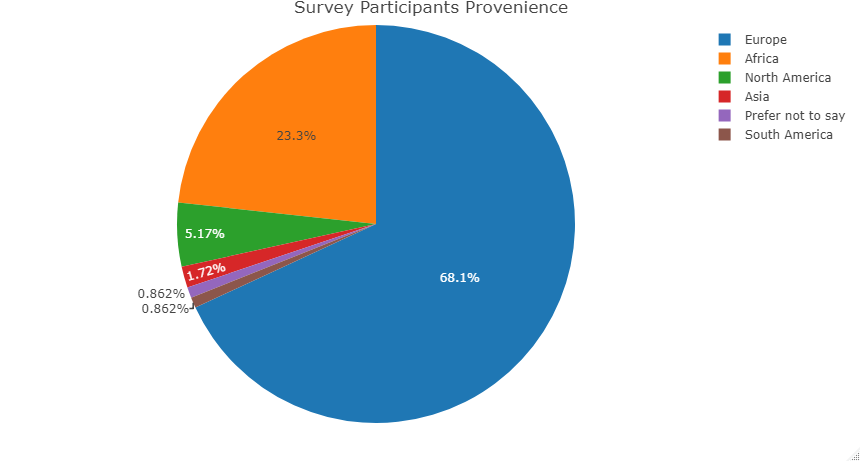
\includegraphics[width=1\textwidth]{figure/Analisi/Background/Survey_Partecipants_Provenience.png}
        \caption{Distribuzione continentale del campione di analisi}
    \end{figure}
    
    Come osservabile dalla figura 5.1, il campione di analisi, è principalmente concentrato tra Europa e Africa, ciò significa appunto che le deduzioni successive, questo dettaglio non è trascurabile, dato che la generalizzabilità dei risultati, potrebbe essere messa in discussione, per aree geografiche rappresentate in maniera minore. Ad ogni modo, questo prima considerazione, è senz'altro da attribuire al fatto che Prolific è essenzialmente una piattaforma di origine britannica, quindi maggiormente pubblicizzata in Europa. Nel dettaglio, 79 partecipanti hanno dichiarato di provenire dall'europa, 27 dall'africa, 6 dal nord america, 2 dall'asia, 1 dal sud america, mentre 1 ha preferito non dichiarare la sua provenienza.
    
    \begin{figure}[h]
        \centering
        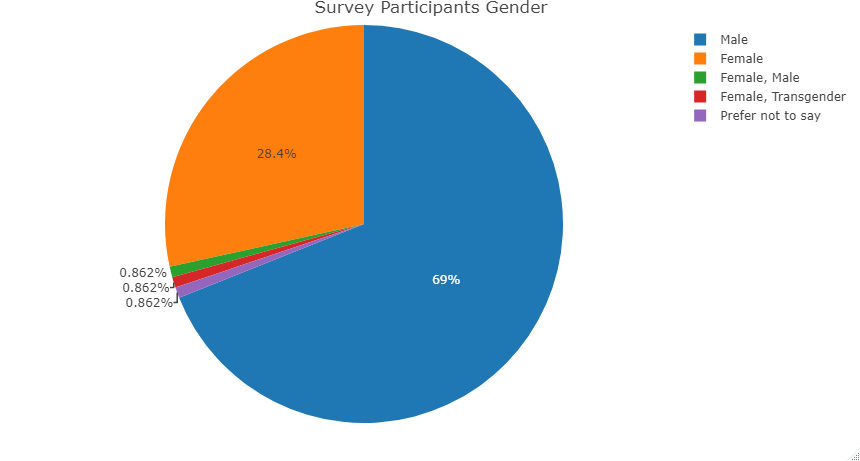
\includegraphics[width=1\textwidth]{figure/Analisi/Background/Survey_Partecipants_Gender.png}
        \caption{Distribuzione di gender nel campione di analisi}
    \end{figure}
    
    Analogamente alla provenienza, con la figura 5.2 è possibile effettuare qualche considerazione analoga, con l'identificazione di gender dei partecipanti. la presenza di tale quesito è stato ampiamente discussa in fase di progettazione del questionario, dato che essa è spesso un informazione da ritenere altamente discriminatoria se non non richiesta nel modo giusto, a tale scopo, è stata introdotta l'opzione di controllo Prefer Not To Say, che tuttavia è stata selezionata solo da un partecipante su 116. 80 invece si identificano nel gender maschile, 33 in in quello femminile, 1 in entrambi i precedenti, 1 come Transgender e donna contemporaneamente.\\
    
    \begin{figure}[h!]
        \centering
        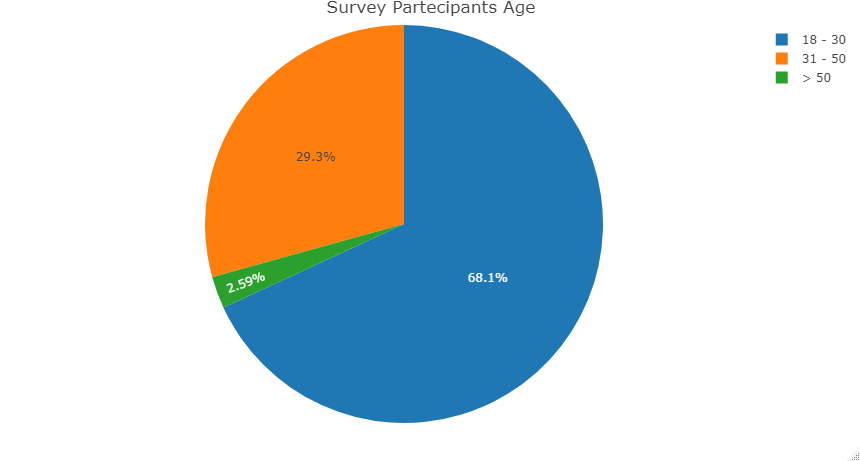
\includegraphics[width=1\textwidth]{figure/Analisi/Background/Survey_Partecipants_Age.png}
        \caption{Distribuzione dell'età nel campione di analisi}
    \end{figure}
    
   Considerando invece la figura 5.3 è possibile notare, come la maggioranza del campione, si concentri maggiormente tra i 18 e i 30 anni, più nello specifico 79 partecipanti si colloca in questo range, 34 invece sono i partecipanti appartenenti alla fascia di età tra i 31 e i 50 anni, portando quindi anche maggiore maturità professionale al campione, mentre infine 3 partecipanti dichiarano di possedere più di 50 anni.
   
   \begin{figure}[h!]
        \centering
        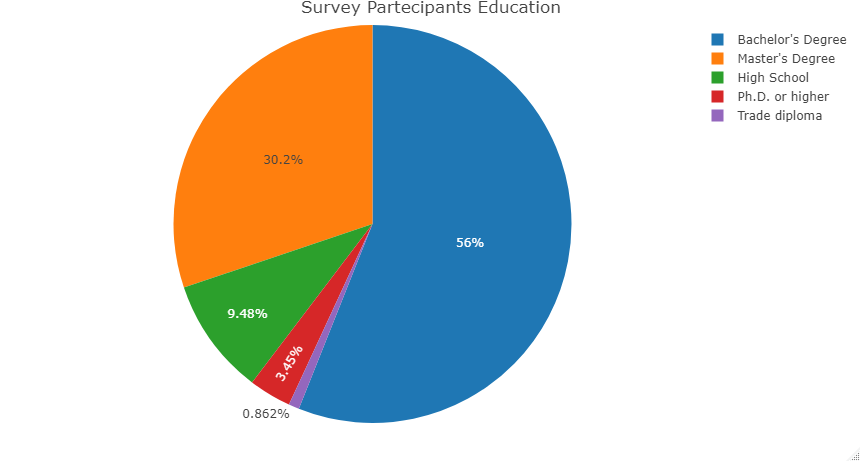
\includegraphics[width=1\textwidth]{figure/Analisi/Background/Survey_Partecipants_Education.png}
        \caption{Distribuzione del livello di studi nel campione di analisi}
    \end{figure}
   Fin dall'inizio della fase di progettazione del Survey, al fine dell'attendibilità delle informazioni ricevute è stata considerato come fattore di rilevante importanza il livello di studio medio dei partecipanti, preferendo in particolare un alto livello di studio (laurea triennale e superiori), dalla figura 5.4 è osservabile come tale tendenza sia rispettata da quasi tutti i partecipanti all'indagine, nel dettaglio su 116 partecipanti totali, 65 dichiarano di possedere almeno un titolo di studi triennale, 35 invece dichiarano di aver conseguito un titolo magistrale, 4 risultano aver completato anche il dottorato di ricerca, mentre i restati 12 si dividono in 11 con un diploma di istruzione superiore e un singolo con diploma professionale.\\
   
   Continuando poi con la posizione e il ruolo professionale dei partecipanti, è possibile notare come effettivamente, il campione degli intervistati sia abbastanza variegato e corrispondente ai requisiti di appartenenza precedentemente fissati. 
   
    \begin{figure}[h!]
        \centering
        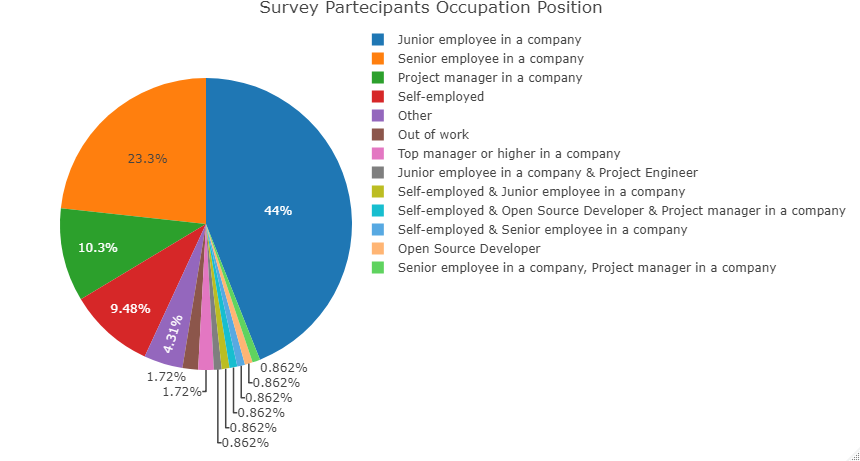
\includegraphics[width=1\textwidth]{figure/Analisi/Background/Survey_Partecipants_Occupation_Position.png}
        \caption{Livello di occupazione professionale dei partecipanti all'analisi}
    \end{figure}
    
    In particolare, come osserva la figura 5.5, la maggioranza dei partecipanti ricopre un ruolo attivo in una compagnia, nel dettaglio è possibile dividere questa fetta in 51 impiegati aziendali junior, 27 impiegati aziendali Senior, e 12 Project Manager e 2 come Top-Manager  in azienda. Tra i restanti, 11 si dichiarano come lavoratori autonomi. Tra i restanti, ci sono figure professionali singole, che dichiarano di ricoprire più di una posizione professionale contemporaneamente o altri ruoli quali sviluppatore open source, infine risultano esserci 5 partecipanti che dichiarano di avere altra posizione altro rispetto a quelle specificate, mentre solo 2 risultano disoccupati al momento della sottomissione.  
    
      \begin{figure}[h!]
        \centering
        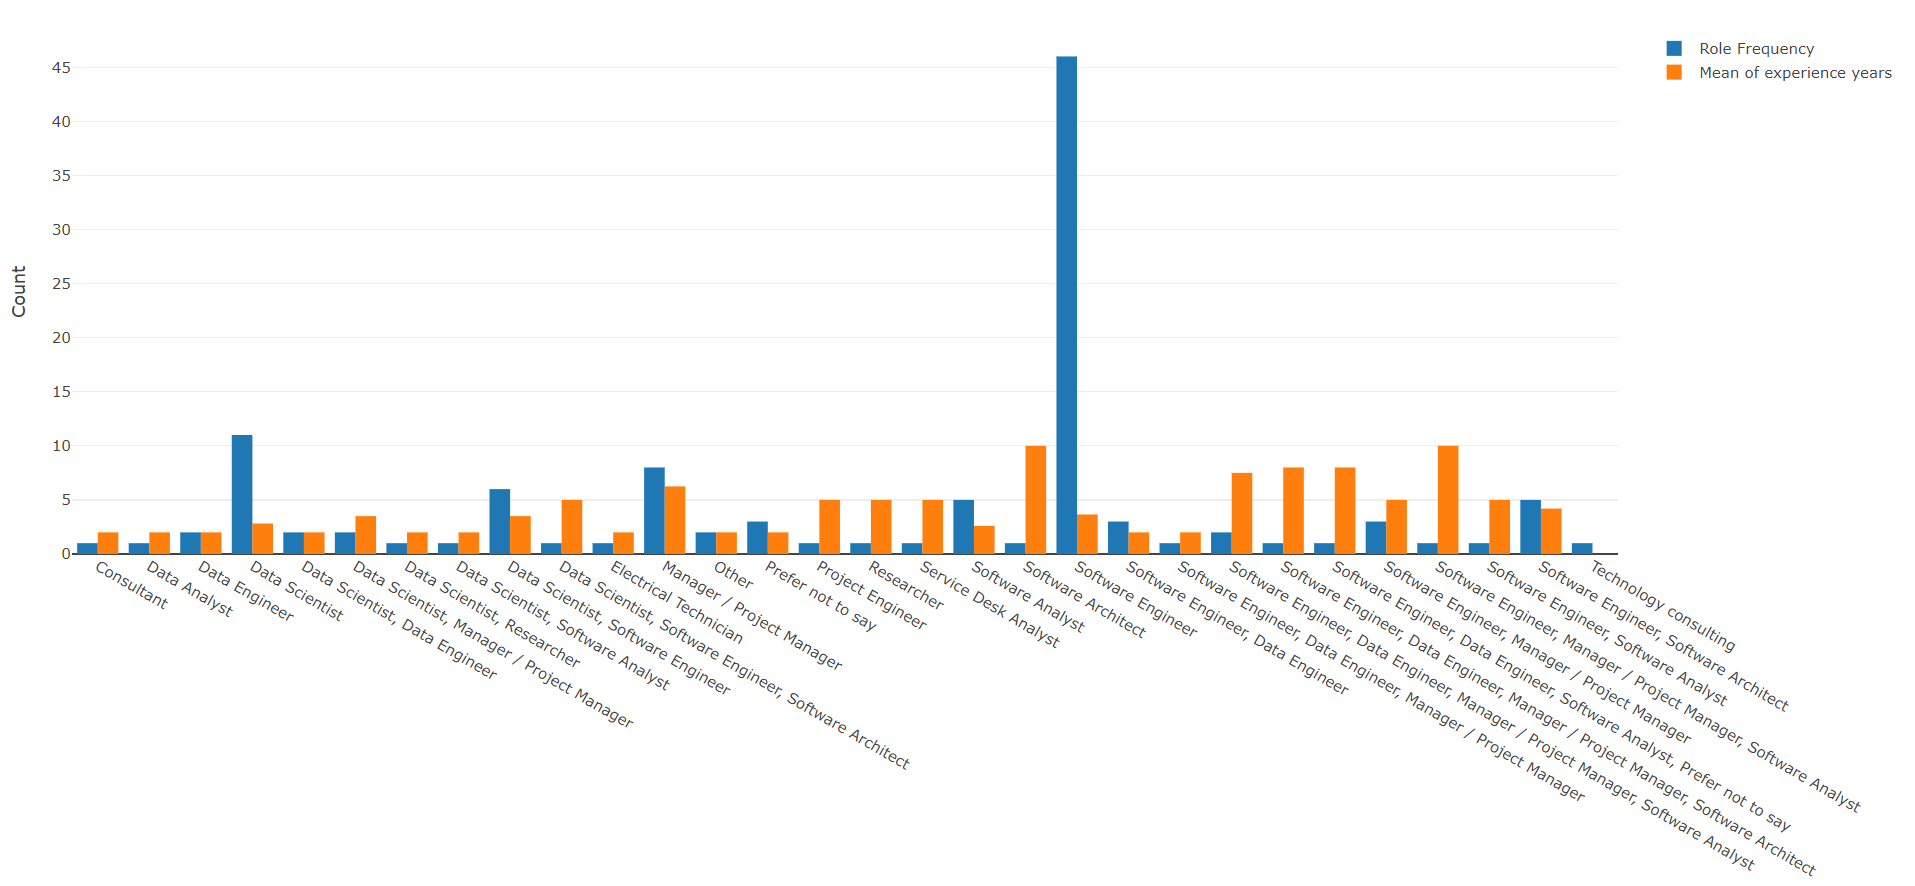
\includegraphics[width=0.8\textwidth]{figure/Analisi/Background/Survey_Partecipants_Roles.png}
        
        \caption{Ruoli professionali dei partecipanti all'analisi}
    \end{figure}
    
    Dando invece uno sguardo ai ruoli professionali, è possibile osservare come circa la metà o poco più dei partecipanti, abbia affinità con l'ingegneria del software, l'ingegneria dei dati, e il management, leggermente meno ampia è la presenza di ruoli affini a posizioni quali Data Science o altri ruoli professionali, mentre in media. Mentre è di rilievo considerare che tutti i partecipanti hanno in media dai 2 ai 10 anni di esperienza nel ruolo indicato. Da un punto di vista empirico, l'eterogeneità del campione è senz'altro molto positiva dato che sia per via dei differenti ruoli, che per i variegati livelli di occupazione, è possibile dare più valenza statistica alle successive informazioni estratte dai dati grezzi.
    
    \subsection{Fairness in pratica, come rispondere al quesito generale?}
    
    
    \begin{center}
		\hspace*{-5mm}\begin{tikzpicture}
			\node [mybox] (box){%
				\begin{minipage}{.70\textwidth}
					\centering
					
                    	\textit{RQ -  In che modo il concetto di Software Fairness è attualmente percepito nell'ambiente lavorativo ML-Intensive?}
				
				\end{minipage}
			};
		\end{tikzpicture}%
	\end{center}
	
	Come più volte osservato più volte, cercar di raccogliere dati utili a rispondere in maniera formale a questo unico macro-quesito, può essere qualcosa di generalmente complesso e forse anche riduttivo da proporre per un concetto così variegato come quello di Software Fairness, sicuramente considerando l'andamento generale dell'analisi dei dati, così come viene riportato nei successivi paragrafi, è senz'altro facile capire che, come stabilito dalla ricerca Fairness, è un concetto estremamente variabile ed in evoluzione, quindi così come per la fase di progettazione, anche quella di analisi risulta essere più assimilabile se scomposta in sotto-punti speculari ai sub-goal di ricerca definiti. 
    
    \subsection{Applicabilità di definizioni e approcci per fairness}
    
    \begin{center}
			\hspace*{-5mm}\begin{tikzpicture}
			\node [mybox] (box){%
				\begin{minipage}{.70\textwidth}
					\centering
					\textit{RQ1 - Quali sono i migliori approcci e definizioni per trattare la fairness in un contesto lavorativo?}
				\end{minipage}
			};
		\end{tikzpicture}%
	\end{center}
    
     \begin{figure}[h!]
        \centering
        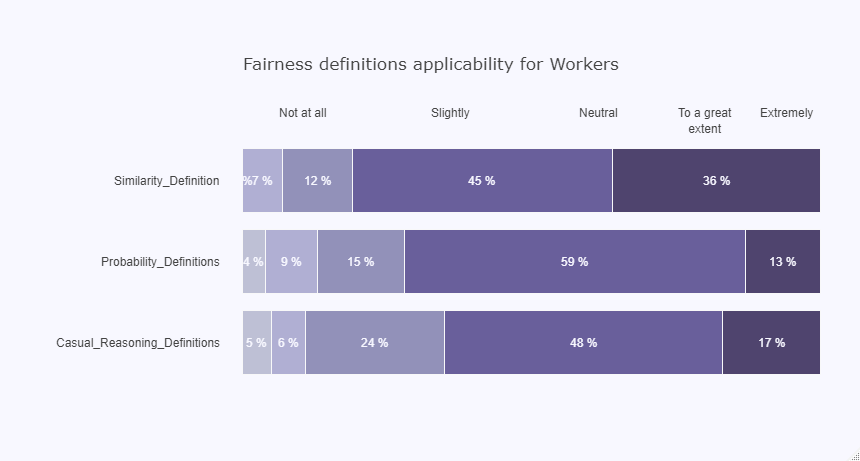
\includegraphics[width=1\textwidth]{figure/Analisi/RQ1/Hist_Fairness_Deginitions_Applicability.png}
        \caption{Definizioni di fairness in ambito lavorativo}
    \end{figure}
    
    Data l'ampia variabilità del concetto, non è corretto porre un quesito di ricerca che voglia definire univocamente il concetto o la definizione \emph{aziendale} di software fairness. Da un punto di vista analitico, la figura 5.7, dimostra infatti come per gli esperti, tutte le tipologie di definizioni e metriche teoriche, possono essere ampiamente applicate in casi reali di sviluppo, per tutte e tre i gruppi di definizione, i livelli 4 e 5 delle scale di applicabilità superano il 50\% dei consensi, a seconda dei contesti di applicazioni e dei requisiti specifici del modulo ML. Da un'analisi più attenta, però si può osservare come i partecipanti all'indagine ritengano lievemente più applicabili i gruppi di definizione e metriche basati su \textbf{similarità matematica}, rispetto a quelli definiti in \textbf{puri termini probabilistici} piuttosto che quelli basati su \textbf{relazioni causali tra features e outcome}.
    
      \begin{figure}[h!]
        \centering
        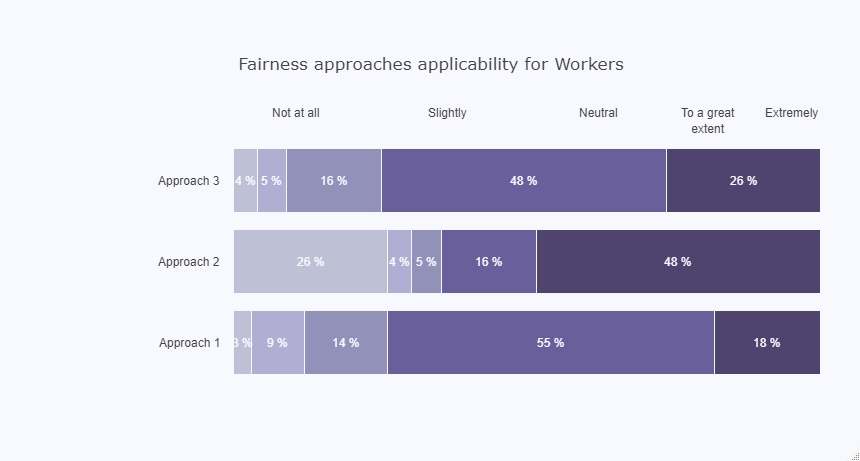
\includegraphics[width=1\textwidth]{figure/Analisi/RQ1/Hist_Fairness_Approaches_Applicability.png}
        \caption{Approcci al concetto di fairness in ambito lavorativo}
    \end{figure}
    
    Contrariamente se si osservano gli approcci pratici proposti, si osserva facilmente come in azienda prevalga facilmente l'idea che \textbf{i livelli alti di Software Fairness}, vadano ricercati cercando di \textbf{ridurre le dipendenze tra gli attributi sensibili e i risultati predetti in fasi di data preparation} (approccio 1), e quindi specularmente nel \textbf{cercare di constatare che i risultati stessi non dipendano da feature sensibili} in fase di validazione (approccio 3). Meno percepito come applicabile, risulta essere invece il secondo approccio proposto, ovvero concentrarsi nel garantire che il learner non effettui valutazioni discriminatorie sulla base di feature sensibili. Ciò è probabilmente da attribuire, alla complessità di questa seconda opzione proposta, non facilmente intuibile e difficilmente analizzabile rispetto le altre due.\\
    
    Ovviamente anche in azienda, il concetto di fairness non si limita a quanto espresso in teoria, esso può essere visto a vari livelli di dettaglio, e soprattutto in riferimento al dominio di utilizzo. A dimostrazione di ciò, risultano interessanti molte risposte ottenute al terzo quesito (risposta aperta breve) progettato per questo primo sub-goal di ricerca, ovvero: Generalmente utilizzi altri approcci per lavorare con il concetto di Software Fairness?
	
	Segue un breve report di alcune delle considerazioni più interessanti:
	
	\begin{itemize}
	    \item Approcci Domain Specific - Provare a rendere i risultati disponibili a persone con disabilità, quindi in sostanza, renderli equi per tutti; 
	    \item Metodologie Empiriche - Condurre survey e ottenere in cosiderazioni opinioni diverse;
	    \item Ottimizzazione nella gestione dei dati - Ottenere dei dati di training sensibili abbastanza affinchè i risultati siano il meno possibile discriminanti;
	    \item Analisi di correlazione - Analizzare la correlazione forte-debole tra risultati e features;
	\end{itemize}
    
	
	
	\begin{center}
	
        \begin{tcolorbox}[width=\textwidth, colframe=black, colback=Gray]
    			\begin{minipage}{\textwidth}
    				\textit{\faKey  \textbf{ Risultato di ricerca 1}}\\
    				In ambienti di sviluppo ML-Intensive, definizioni e metriche formali basate su similarità matematica risultano essere lievemente più utilizzate di altre basate su puro calcolo probabilistico o relazioni causali nel trattamento di fairness come specifica di qualità.
    			
    			\end{minipage}
		\end{tcolorbox}
	\end{center}
	
	\begin{center}
	
        \begin{tcolorbox}[width=\textwidth, colframe=black, colback=Gray]
    			\begin{minipage}{\textwidth}
    				\textit{\faKey  \textbf{ Risultato di ricerca 2}}\\
    				Tra gli approcci pratici per il trattamento di fairness in un modulo ml-intensive, approcci di data preparation e analisi delle prestazioni basati su riduzione delle dipendenze tra feature sensibili e risultati risultano essere lievemente più applicabili rispetto analisi di configurazione basate direttamente su predizioni discriminatorie del modello.
    			
    			\end{minipage}
		\end{tcolorbox}
	\end{center}
	
	\begin{center}
	
        \begin{tcolorbox}[width=\textwidth, colframe=black, colback=Gray]
    			\begin{minipage}{\textwidth}
    				\textit{\faKey  \textbf{ Risultato di ricerca 3}}\\
    			  Il trattamento di fairness è gestito in azienda anche con altre metodologie meno note e sistematizzate dallo stato attuale della letteratura, vengono infatti suggerite, dai professionisti, altre pratiche di rilievo, e.g. metodologie empiriche, correlazione statistica o ottimizzazione nella gestione dati.
    			
    			\end{minipage}
		\end{tcolorbox}
	\end{center}
	
    \subsection{Impatto professionale per il trattamento della fairness}
	\begin{center}
		\hspace*{-5mm}\begin{tikzpicture}
			\node [mybox] (box){%
				\begin{minipage}{.70\textwidth}
					\centering
					\textit{RQ2 - Come è composto generalmente un team lavorativo per lo sviluppo di moduli ML-Intensive Fair Critical?}
				\end{minipage}
			};
		\end{tikzpicture}%
	\end{center}
	
	  \begin{figure}[h!]
        \centering
        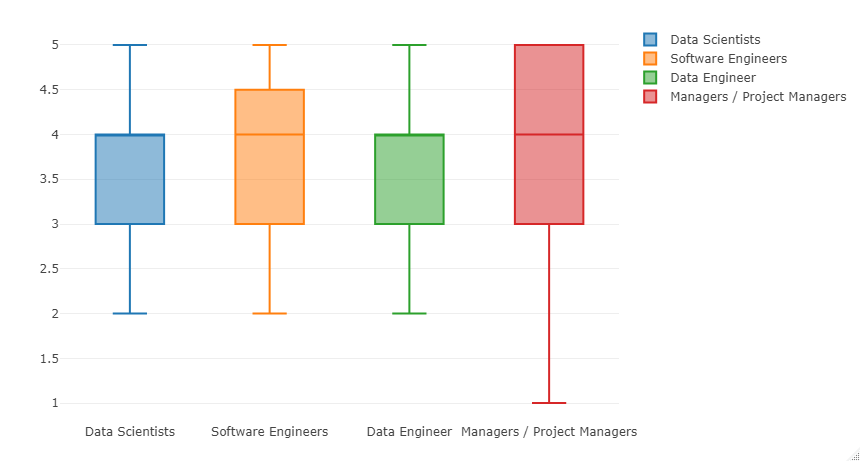
\includegraphics[width=1\textwidth]{figure/Analisi/RQ2/RoleImpactBoxPlot1.png}
        \caption{Ruoli professionali durante lo sviluppo Fair Oriented 1/2}
    \end{figure}
    
     \begin{figure}[h!]
        \centering
        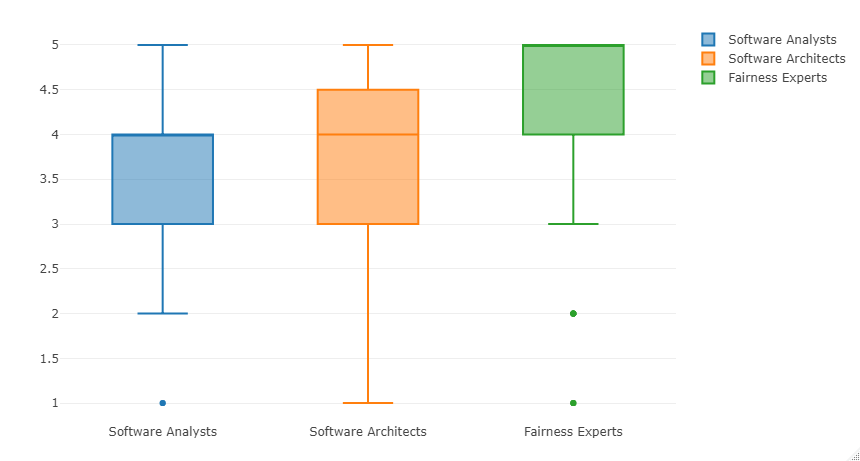
\includegraphics[width=1\textwidth]{figure/Analisi/RQ2/RoleImpactBoxPlot2.png}
        \caption{Ruoli professionali durante lo sviluppo Fair Oriented 2/2}
    \end{figure}
	 
	 
	 Osservando le figure 5.9 e 5.10, è facilmente intuibile, come \textbf{tutti i ruoli professionali} proposti,vengano considerati cruciali durante lo sviluppo di una soluzione fair critical, infatti il valore mediano per ogni figura professionale si attesta almeno a 4 (secondo valore di rilevanza nella scala precedentemente illustrata). Volendo entrare più nel dettaglio, è possibile osservare come \textbf{manager} ed \textbf{esperti specifici}, siano figure estremamente di rilievo e utili nella gestione degli aspetti di equità di un modulo di Machine Learning. Risultano molto simili sono invece attribuibili a figure come Data Scientist, Data Engineer e Ingegneri del software, a dimostrazione del fatto che, anche in un contesto reale, mantenere alta la sinergia tra queste due branche dello sviluppo ML-Intensive sia cruciale soprattutto in contesti molto specifici come quello della fairness. Da notare come ci sia una leggera presenza di outliers per ruoli come Analisti ed Esperti di fairness (basso impatto in controtendenza con il resto del campione), ma ciò è da considerare come fattore eccezionale, dato che tali figure possono essere comunque molto specifiche e magari non presenti in ogni ambiente lavorativo dei partecipanti all'indagine.
	 
	 
	 \begin{center}
	
        \begin{tcolorbox}[width=\textwidth, colframe=black, colback=Gray]
    			\begin{minipage}{\textwidth}
    				\textit{\faKey  \textbf{ Risultato di ricerca 4}}\\
    			 Per la gestione di problematiche etiche durante lo sviluppo di moduli di machine learning, risulta essenziale l'adozione di accurate strategie di management, viene indicato infatti come le figure manageriali siano particolarmente critiche nel trattamento di fairness.
    			\end{minipage}
		\end{tcolorbox}
	\end{center}
	
	\begin{center}
	
        \begin{tcolorbox}[width=\textwidth, colframe=black, colback=Gray]
    			\begin{minipage}{\textwidth}
    				\textit{\faKey  \textbf{ Risultato di ricerca 5}}\\
    			 Per la gestione di problematiche etiche durante lo sviluppo di moduli di machine learning, risulta essenziale il coinvolgimento di esperti specifici.
    			\end{minipage}
		\end{tcolorbox}
	\end{center}
	

	
	\begin{center}
	
        \begin{tcolorbox}[width=\textwidth, colframe=black, colback=Gray]
    			\begin{minipage}{\textwidth}
    				\textit{\faKey  \textbf{ Risultato di ricerca 6}}\\
    			 Durante lo sviluppo di moduli di machine learning, per la gestione qualitativa di fairness, risulta equiparabile la rilevanza nel team di figure professionali trasversali, quali Data Scientist, Ingegneri del Sotfware, Analisti etc.
    			\end{minipage}
		\end{tcolorbox}
	\end{center}
    \subsection{Confronto tra fairness con altre caratteristiche qualitative non funzionali}
    
    \begin{center}
		\hspace*{-5mm}\begin{tikzpicture}
			\node [mybox] (box){%
				\begin{minipage}{.70\textwidth}
					\centering
					\textit{RQ3 - Quanto il concetto di software fairness è importante se paragonato ad altri aspetti non funzionali?}
				\end{minipage}
			};
		\end{tikzpicture}%
	\end{center}
	Come visto più volte, analizzare la fairness, come un vero e proprio attributo non funzionale di prima classe sia la chiave di lettura al fine di eliminare fault etici latenti in un modulo di machine learning \cite{brun2018software}. Ovviamente chiedere richiedere tale sforzo ai professionisti è un qualcosa di molto ostico soprattutto mettendo a paragone Fairness, con requisiti molto più standardizzati, quali accuracy o sicurezza. Ma analizzando i risultati, è possibile provare ad osservare qualche deduzione interessante.\\
	
	N.B. nei successivi diagrammi, sono state rappresentate le densità delle singole risposte dei partecipanti, in blu si può notare la fetta di persone che considera uno specifico requisito altamente meno importante rispetto a Fairness (-2 della scala quantitativa) , in verde è racchiusa la parte di campione che considera fairness leggermente più importate rispetto all'altro requisito analizzato dal diagramma (-1 della scala quantitativa), in giallo quella che considera fairness rilevante quanto il requisito confrontato (0 nella scala quantitativa), in arancione quella fetta di campione che considera il requisito in analisi lievemente più importante rispetto a fairness (+1), mentre in rosso gli individui che considerano il requisito specifico altamente più importante di fairness (+2).
	\begin{figure}[h!]
        \centering
        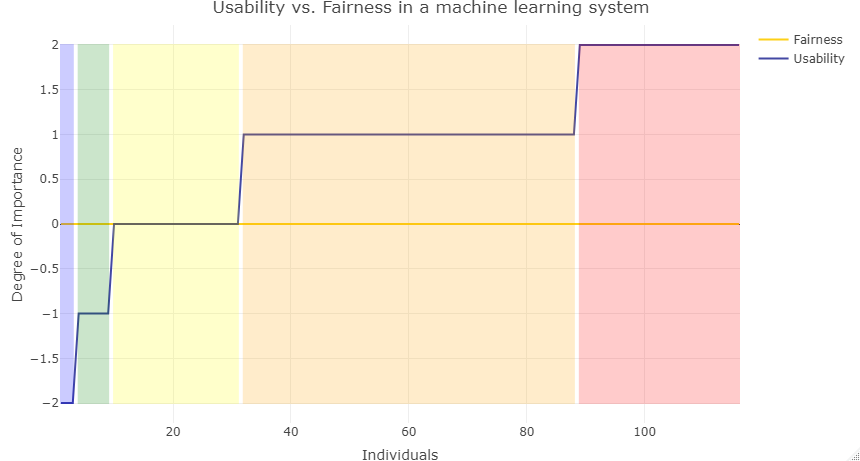
\includegraphics[width=1\textwidth]{figure/Analisi/RQ3/1.Usability_vs_Fairness.png}
        \caption{Fairness vs Usabilità}
    \end{figure}
    
    \begin{figure}[h!]
        \centering
        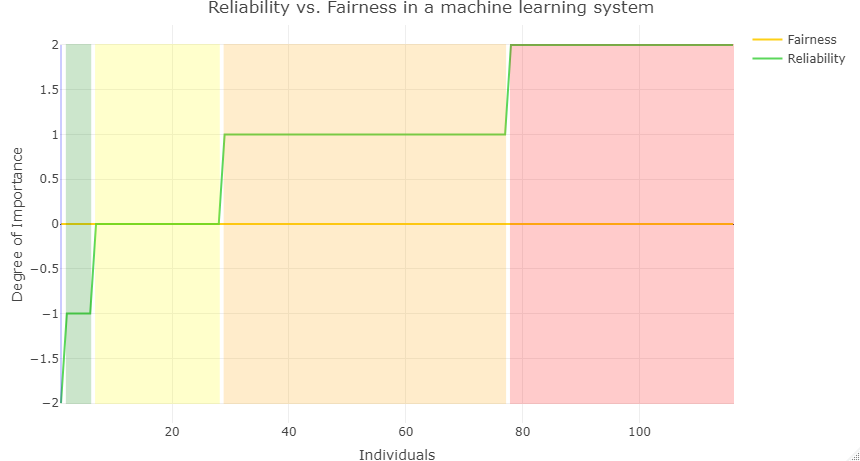
\includegraphics[width=1\textwidth]{figure/Analisi/RQ3/2.Reliability_vs_Fairness.png}
        \caption{Fairness vs Affidabilità}
    \end{figure}
    
    \begin{figure}[h!]
        \centering
        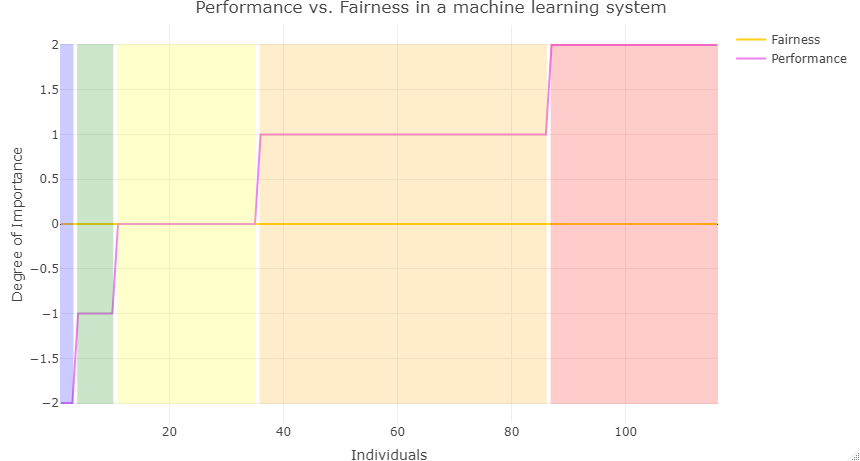
\includegraphics[width=1\textwidth]{figure/Analisi/RQ3/3.Performance vs. Fairness.png}
        \caption{Fairness vs Performances}
    \end{figure}
    
    
    \begin{figure}[h!]
        \centering
        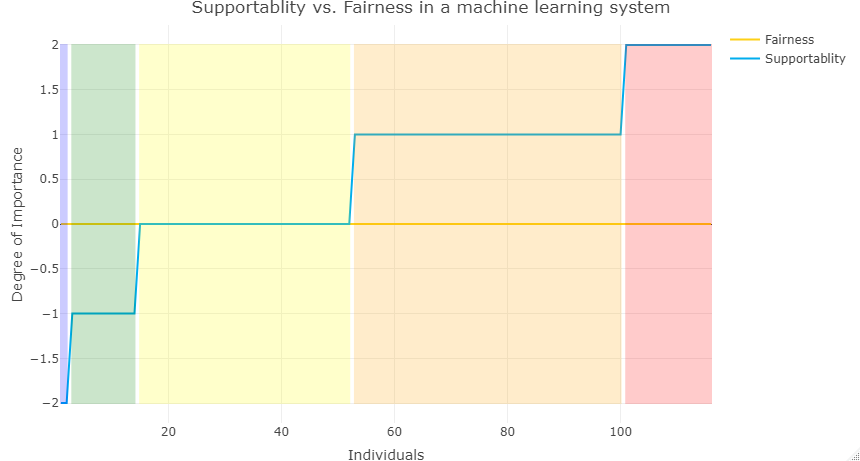
\includegraphics[width=1\textwidth]{figure/Analisi/RQ3/4.Supportablity vs. Fairness.png}
        \caption{Fairness vs Supportabilità}
    \end{figure}
    
    
    Come osservabile dalle figure 5.11 alla 5.14, aspetti non funzionali standard, del noto modello furps+ (usabilità, affidabilità, performance e supportabilità), sono aspetti che per la maggior parte del campione, risultano essere di misura più rilevanti di fairness, in particolare si osserva che per aspetti particolarmente critici per i moduli di intelligenza artificiale, quali \textbf{affidabilità e performances}, la fetta di persone che li considera \textbf{estremamente più importanti}, sale anche \textbf{sopra le 25/30 unità}, per diminuire leggermente negli altri aspetti riportati. È però da tener conto come quasi tutti gli aspetti del modello iniziale analizzato (Furps+), come fairness, siano altamente variabili a seconda delle necessità del tool specifico, infatti, osservando come la maggior parte dei partecipanti consideri \textbf{usabilità e supportabilità} leggermente più impattanti nello sviluppo ml-intensive, rispetto fairness, si può sicuramente lasciare margine di confronto tra questi attributi e fairness a seconda delle specifiche esigenze.
    \begin{figure}[h!]
        \centering
        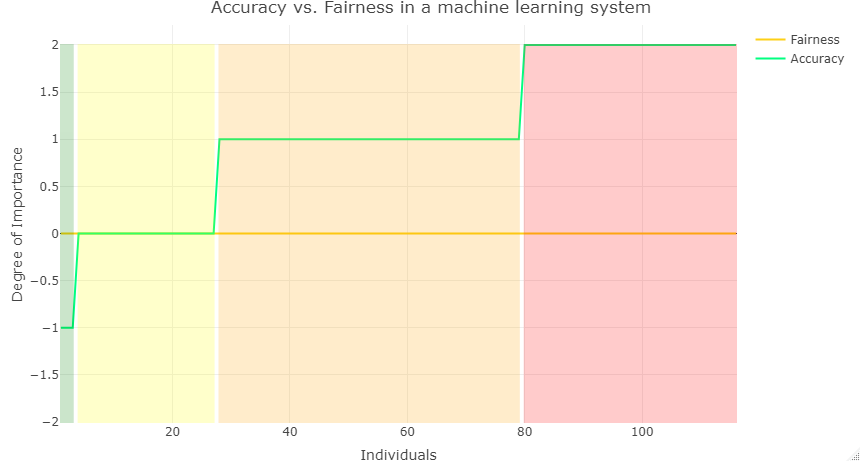
\includegraphics[width=1\textwidth]{figure/Analisi/RQ3/5.Accuracy vs. Fairness.png}
        \caption{Fairness vs Accuracy}
    \end{figure}
    
     \begin{figure}[h!]
        \centering
        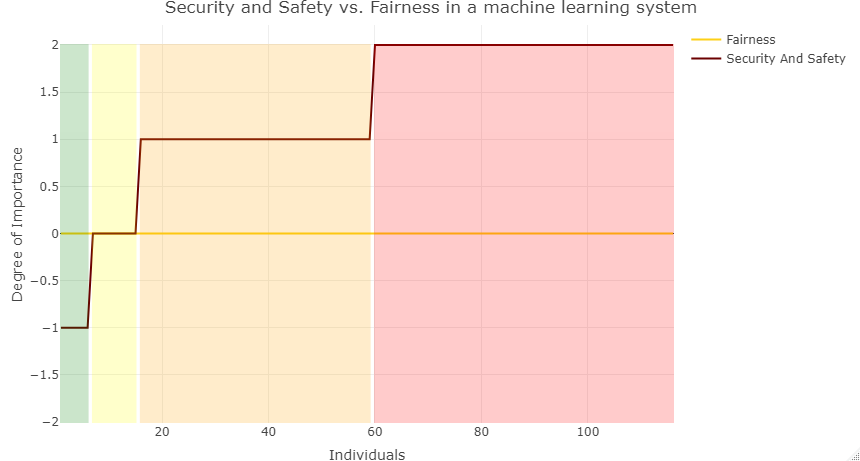
\includegraphics[width=1\textwidth]{figure/Analisi/RQ3/6.Security and Safety.png}
        \caption{Fairness vs Sicurezza}
    \end{figure}
    
    Il discorso cambia di misura per aspetti già più specifici per un canonico modello di machine learning, infatti sia per accuracy che sicurezza, nessuno dei partecipanti ha ritenuto opportuno indicarli come ampiamente meno importanti rispetto alla fairness, inoltre per questi due aspetti anche la finestra di voto che va da -1 a 0, risulta essere molto ristretta. Sia \textbf{l'accuracy che la Sicurezza, sono da considerare da lievemente ad estremamente più rilevanti} rispetto a fairness sulla base del campione. Ciò molto probabilmente è dovuto al fatto che chi lavora quotidianamente con questi sistemi, in maniera quasi automatica si troverà a lavorare a problematiche di accuracy o sicurezza del modello, cosa non sempre così semplice (almeno allo stato attuale delle cose) per fairness. 
    \begin{figure}[h!]
        \centering
        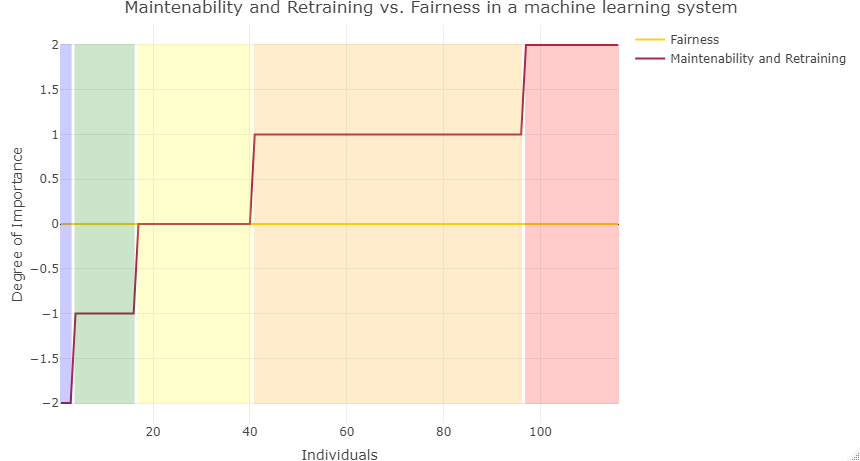
\includegraphics[width=1\textwidth]{figure/Analisi/RQ3/7.Maintenability and Retraining.png}
        \caption{Fairness vs Manutenibilità e Retraining}
    \end{figure}
    
    \begin{figure}[h!]
        \centering
        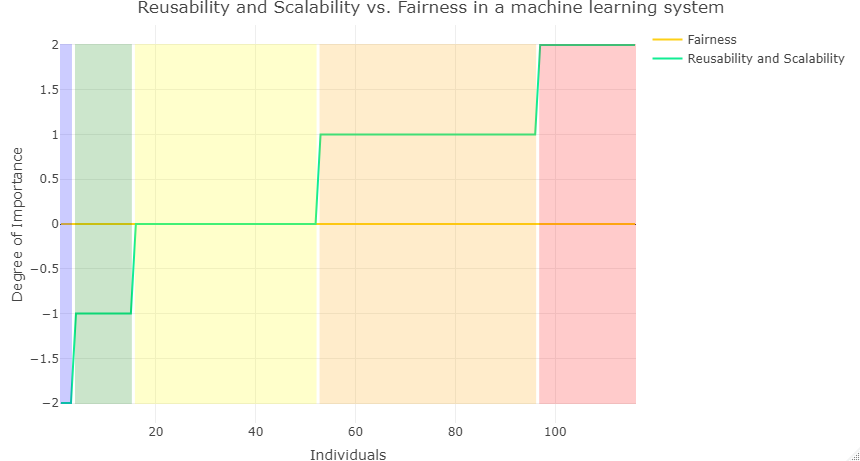
\includegraphics[width=1\textwidth]{figure/Analisi/RQ3/8.Reusability and Scalability.png}
        \caption{Fairness vs Riusabilità e Scalabilità}
    \end{figure}
    
    In maniera più semplificata (aggregando i concetti), è stato chiesto ai partecipanti di provare a fornire un parere similare alle altre specifiche non funzionali quali manutenibilità \& retraining - figura 5.17 (in ottica evolutiva di un generico tool ML-Intensive) e scalabilità \& riusabilità - figura 5.18. Per questa tipologia di requisiti, i report grafici, possono facilmente far dedurre considerazioni similari rispetto al modello Furps+, ma probabilmente per arrivare ad osservazioni più precise, si dovrebbe analizzare separatamente i singoli dati (scelta non adottata per evitare di rendere troppo complesso il quesito ai partecipanti).\\\\
    
    In generale, le problematiche discriminatorie ed il concetto di software fairness, sono probabilmente concetti molto distanti dagli aspetti di qualità, già ampiamente studiati e sistematizzati. Allo stato della pratica, il generico lavoratore, sia esso data scientist, ingegnere del software, manager o quant'altro, difficilmente darà  più rilevanza in termini assoluti a fairness rispetto ad altre prerogative non funzionali (a maggior ragione per aspetti critici, quali accuracy, performance o sicurezza), e le cause possono essere molteplici, ad esempio:
    
    \begin{itemize}
        \item Probabilmente la rilevanza del concetto di fairness aumenterà mano a mano che la società percepirà le problematiche connesse come un problema prioritario, quindi tali confronti dovranno essere ripetuti in futuro;
        \item Fairness probabilmente necessita di essere analizzata in maniera diversa rispetto gli aspetti non funzionali standard, probabilmente in ragione alla specificità del dominio;

    \end{itemize}
    
    
    Avendo quindi osservato, come gli altri aspetti non funzionali, tendano ad essere considerabili da lievemente più rilevanti a nettamente più rilevanti rispetto la software fairness, considerando l'intero campione di analisi, è possibile provare a formalizzare qualche considerazione ulteriore, analizzando le risposte medie ottenute per singolo settore.\\\\ 
    \emph{N.B: Il singolo valore di confronto tra fairness ed un altro generico NFR, è stato calcolato come media matematica delle singole risposte dello specifico settore}, ad esempio se nella figura 5.19, per il settore Healthcare, è riportato valore 0 della scala quantitativa tra il confronto tra Fairness e Usability, è necessario considerare che \emph{mediamente} per il settore specifico l'aspetto non funzionale Usability è egualmente importante rispetto l'aspetto di Fairness nell'utilizzo/sviluppo di una soluzione ml-intensive.
    

    
    \begin{figure}[h!]
        \centering
        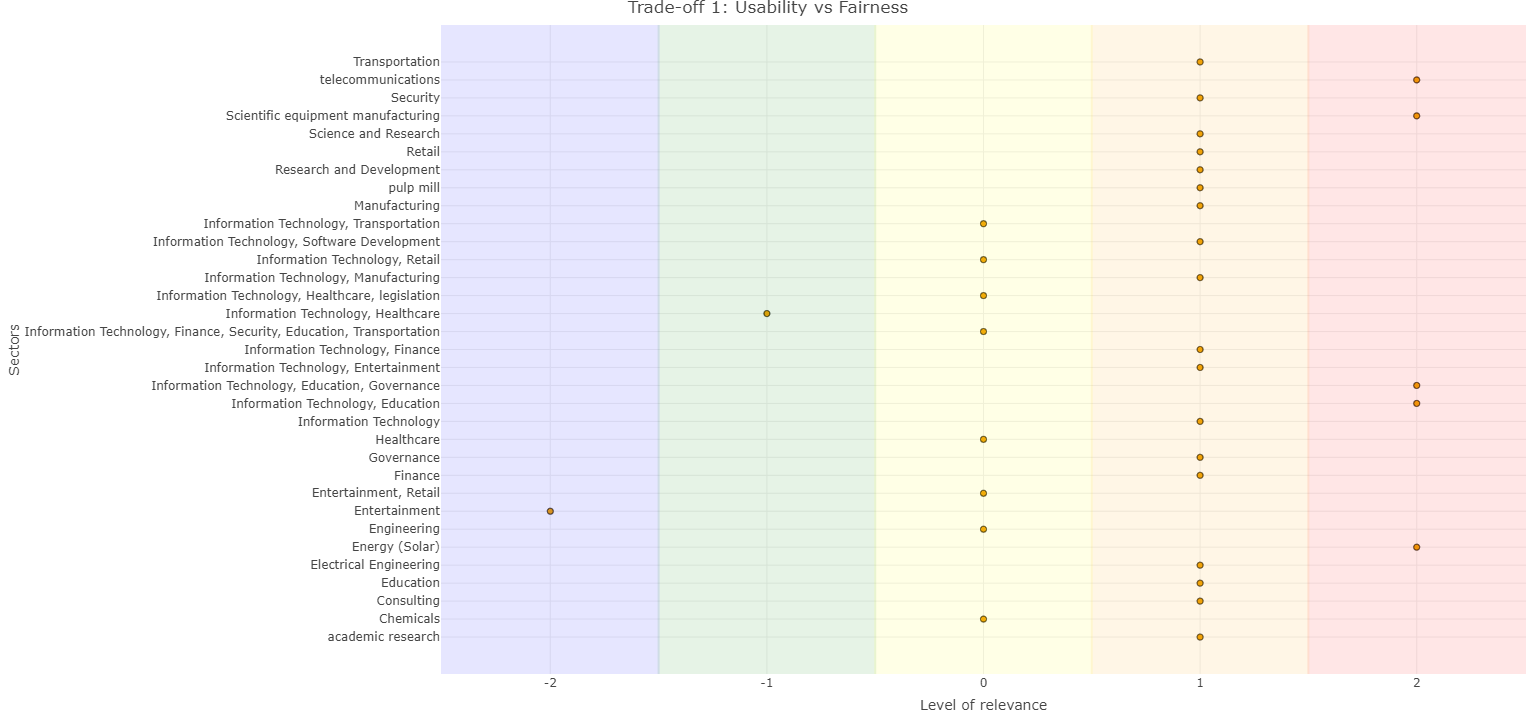
\includegraphics[width=1\textwidth]{figure/Analisi/RQ3/TradeOffsBySectors/1. UsabilityVsFairness.png}
        \caption{Fairness vs Usabilità per settore professionale}
    \end{figure}
    
    L'analisi di dettaglio per settore è disponibile online al link: \url{https://github.com/CFerrara98/Empirical-Investigation-On-Fairness-Development}. Per porre qualche considerazione ulteriore, sono state riportati: il diagramma inerente il confronto tra Usabilità e Fairness - figura 5.19 (rappresentativo della tendenza di risposta che hanno assunto i confronti specifici tra fairness e aspetti qualitativi più comuni tra i moduli Ml Intensive e altri sistemi IT,  e il grafico di confronto per settore tra Sicurezza e Fairness - figura 5.20, rappresentativo della tendenza di confronto assunta per aspetti non funzionali più tecnici in un modulo ML-Intensive.
    
    \begin{figure}[h!]
        \centering
        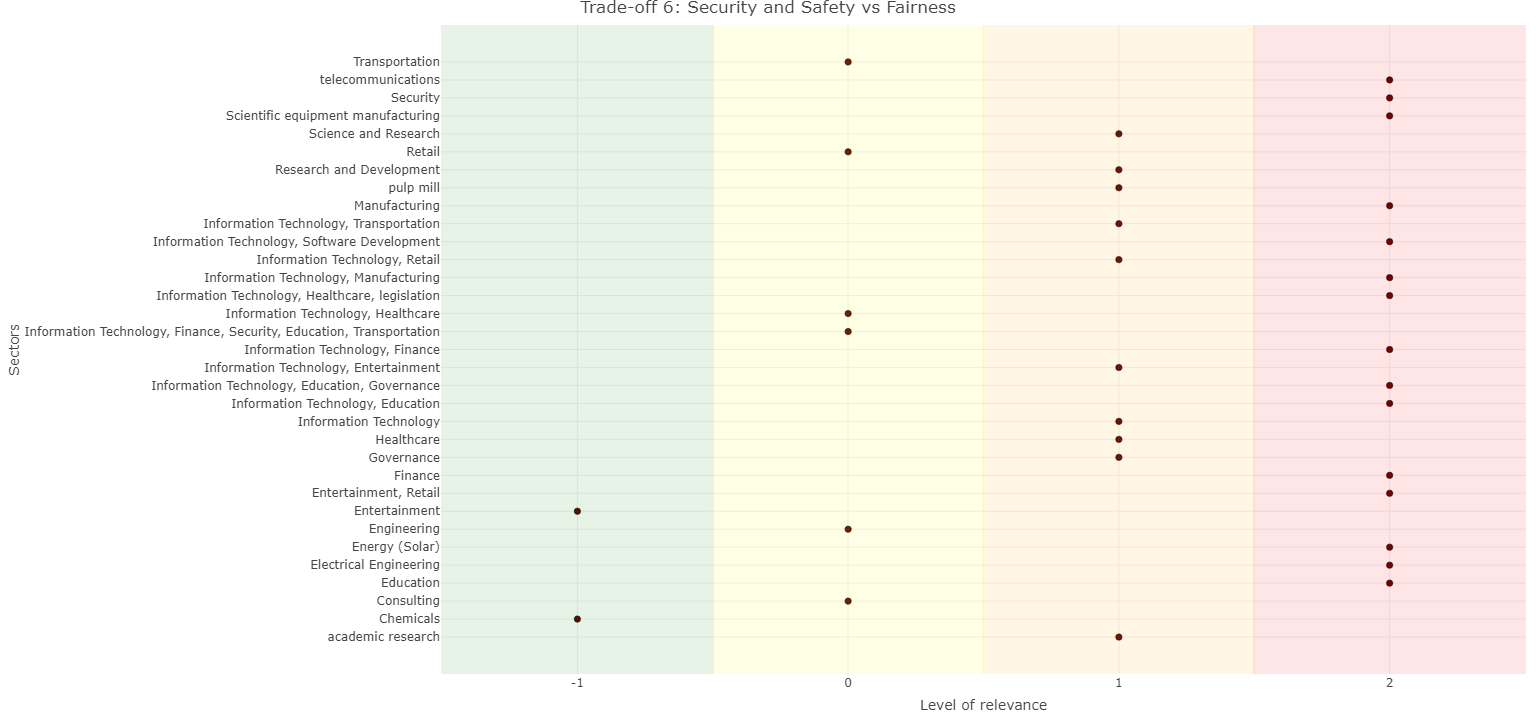
\includegraphics[width=1\textwidth]{figure/Analisi/RQ3/TradeOffsBySectors/6.SecurityAndSafetyVsFairness.png}
        \caption{Fairness vs Sicurezza per settore professionale}
    \end{figure}
    
    Analizzando quindi i \emph{trade-off} non funzionali raggruppando le risposte per settore, si evidenzia quindi come sia confermata la tendenza generale, ovvero che aspetti non funzionali più standardizzati tendono ad essere considerati dalla maggioranza del campione da lievemente più rilevanti ad estremamente più rilevanti, specialmente quando si parla di requisiti criticamente importanti per il buon funzionamento di un modulo ml-intensive e.g. l'aspetto di Sicurezza. Aumentando la granularità del confronto di rilevanza tra fairness e l'altro NFR considerato a livello settoriale, è però possibile porre qualche considerazione più rilevante, è il caso del confronto tra Sicurezza e Fairness, dove si evidenzia una criticità estremamente rilevante della prima rispetto la seconda per settori in cui lavorare in maniera priva di attacchi esterni è estremamente critico o addirittura vitale, e.g. il settore Governance, mentre lo stesso non può dirsi per settori dove gli aspetti di Sicurezza diventano estremamente meno rilevanti rispetto le discriminazioni dell'individuo, è il caso del settore dell'intrattenimento, dove Fairness è considerata addirittura lievemente più rilevante rispetto gli aspetti qualitativi di sicurezza, quasi in contro tendenza con gli altri settori specifici di analisi. \\\\
    
    Ovviamente la tendenza generale dei risultati per questo specifico goal di ricerca resta la stessa rispetto quella osservata a livello generale, ma porre l'accento su esempi di questo tipo, fornisce senz'altro una visione alternativa che fa intendere come fairness possa essere considerato un aspetto prioritario o meno rispetto altri aspetti qualitativi a seconda dello specifico dominio di utilizzo del modulo di machine learning in sviluppo.
    
    \begin{center}
	
        \begin{tcolorbox}[width=\textwidth, colframe=black, colback=Gray]
    			\begin{minipage}{\textwidth}
    				\textit{\faKey  \textbf{ Risultato di ricerca 7}}\\
    			L'etica di un modulo ML-Intensive, sulla base del campione di indagine, risulta essere un aspetto meno rilevante nello sviluppo ML-Intensive se paragonata ad altre specifiche non funzionali meno standardizzate.
    			\end{minipage}
		\end{tcolorbox}
	\end{center}
	
	\begin{center}
	
        \begin{tcolorbox}[width=\textwidth, colframe=black, colback=Gray]
    			\begin{minipage}{\textwidth}
    				\textit{\faKey  \textbf{ Risultato di ricerca 8}}\\
    			La rilevanza media di fairness in un modulo ML-Intensive varia in maniera significativa in funzione della specifica funzionale con cui si effettua il confronto, dai casi in cui fairness risulta essere lievemente meno rilevante (e.g. nel confronto tra fairness e usabilità) fino estremamente meno rilevante (e.g. nel caso tra fairness e sicurezza).
    			\end{minipage}
		\end{tcolorbox}
	\end{center}
	
	\begin{center}
	
        \begin{tcolorbox}[width=\textwidth, colframe=black, colback=Gray]
    			\begin{minipage}{\textwidth}
    				\textit{\faKey  \textbf{ Risultato di ricerca 9}}\\
    			I confronti di rilevanza tra etica ed altre specifiche non funzionali di un modulo di machine learning, risultano assumere risultati medi differenti se l'analisi viene effettuata tenendo conto del settore lavorativo per cui il modulo stesso è progettato.
    			\end{minipage}
		\end{tcolorbox}
	\end{center}
	
    \subsection{Fairness come aspetto intrinseco di una pipeline ML}

    	\begin{center}
    	\hspace*{-5mm}\begin{tikzpicture}
    		\node [mybox] (box){%
    			\begin{minipage}{.70\textwidth}
    				\centering
    				\textit{RQ4 - In quali fasi di una tipica pipeline di Machine Learning è importante adottare strategie per garantire alti livelli di fairness?}
    			\end{minipage}
    		};
    	\end{tikzpicture}%
    \end{center}
    
     \begin{figure}[h!]
        \centering
        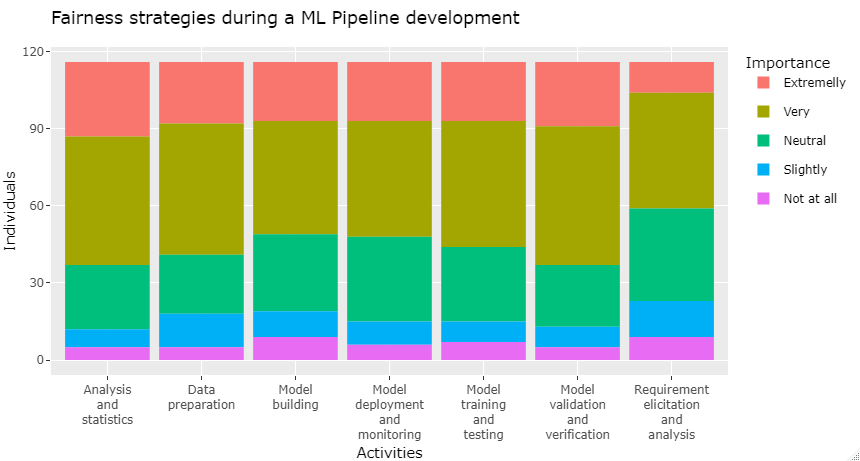
\includegraphics[width=1\textwidth]{figure/Analisi/RQ4/Fairness strategies during a ML Pipeline development.png}
        \caption{Applicabilità di strategie di Fairness improoving in una Pipeline di Machine learining}
    \end{figure}
    Come già osservato in fase di progettazione, questo specifico sub goal, mira a valutare l'utilità di adottare strategie di fairness level improoving in ogni fase di una generica pipeline di machine learning. Dai dati e dal report grafico di figura 5.21, è  evidenziabile, come la \textbf{fairness di un sistema di machine learning è un aspetto di rilevanza in ogni fase di una generica pipeline}, ma da un occhiata più specifica, è facile dedurne come essa stessa può essere un aspetto qualitativo che migliora mano a mano che il sistema evolve sia dopo la fase di building, \textbf{dato che la fase di verifica e validazione viene considerata una delle più valide} per attestare il livello di fairness del sistema, \textbf{seguita dalla fase di analisi e statistica} (successiva al deploy del modello), e di conseguenza dalla \textbf{fase di preparazione dei dati}, che ovviamente va raffinata ad ogni ciclo di sviluppo di una tipica pipeline ML. Ciò significa che la pratica lavorativa, secondo i dati raccolti, probabilmente suggerisce che attualmente la Fairness è un aspetto di un modello di machine learning che va di pari passo con la sua evoluzione, ed è probabilmente lì che è necessario investire con soluzioni specifiche.
    
    \begin{figure}[h!]
        \centering
        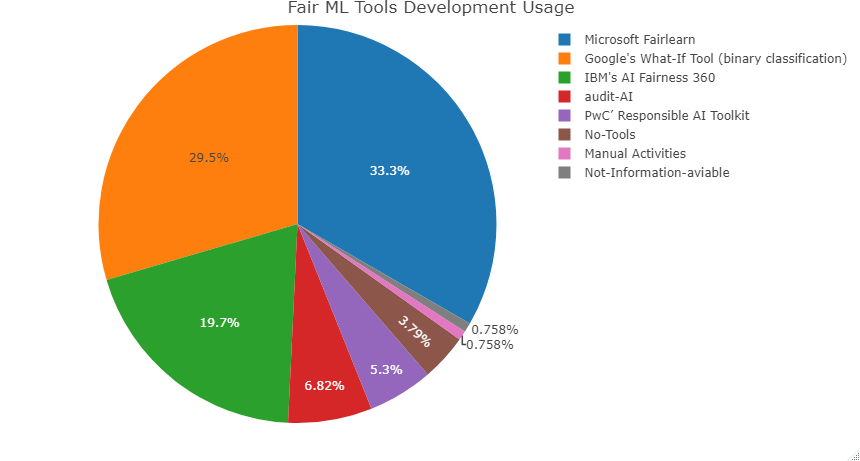
\includegraphics[width=0.9\textwidth]{figure/Analisi/RQ4/Fair ML Tools Development Usage.png}
        \caption{Utilizzo di tool noti per il Fair ML Development}
    \end{figure}
    
    Per fornire altri dettagli circa l'utilizzo di approcci e strumenti utili al trattamento di fairness come aspetto integrante del ciclo di sviluppo di un modulo ml, si osserva (figura 5.22) letteralmente pochi partecipanti all'indagine abbiano fatto dichiarato di non fare uso di tool specifici per il fairness improoving. la maggior parte di essi invece dichiara di aver utilizzato almeno una volta un tool proprietario tra i noti Microsoft Fairlearn, Google's-What-IF o IBM's AI Fairness 360. Ciò è sicuramente un buon segnale, dato che le aziende evidentemente, sono molto propense ad adottare strategie specifiche per progettare soluzioni ML Fair su larga scala.
    
    \begin{center}
	
        \begin{tcolorbox}[width=\textwidth, colframe=black, colback=Gray]
    			\begin{minipage}{\textwidth}
    				\textit{\faKey  \textbf{ Risultato di ricerca 10}}\\
    		     Considerando una canonica pipeline di machine learning, è evidente come l'adottare strategie specifiche per il trattamento di fairness sia particolarmente utile in ogni fase formale di sviluppo.
    			\end{minipage}
		\end{tcolorbox}
	\end{center}
	
	\begin{center}
	
        \begin{tcolorbox}[width=\textwidth, colframe=black, colback=Gray]
    			\begin{minipage}{\textwidth}
    				\textit{\faKey  \textbf{ Risultato di ricerca 11}}\\
    		     Tra le varie fasi di sviluppo di una pipeline di machine learning, gli esperti del dominio considerano lievemente più importanti, nel trattare fairness, quelle che caratterizzano gli aspetti evolutivi del modello, ovvero: le fasi di data praparation, le strategie di verifica e validazione ed analisi e statistiche con il modello in esercizio.
    			\end{minipage}
		\end{tcolorbox}
	\end{center}
	
	\begin{center}
	
        \begin{tcolorbox}[width=\textwidth, colframe=black, colback=Gray]
    			\begin{minipage}{\textwidth}
    				\textit{\faKey  \textbf{ Risultato di ricerca 12}}\\
    		     L'utilizzo di tools e strategie automatiche per il trattamento di fairness, risulta essere ampiamente utile secondo i professionisti. Nello specifico risultano ampiamente utilizzati prodotti specifici di grandi multinazionali, quali IBM, Microsoft e Google.
    			\end{minipage}
		\end{tcolorbox}
	\end{center}
	
    \subsection{Fairness e maturità aziendale}
    
    \begin{center}
    	\hspace*{-5mm}\begin{tikzpicture}
    		\node [mybox] (box){%
    			\begin{minipage}{.70\textwidth}
    				\centering
    				\textit{RQ5 - Quanto le compagnie di sviluppo ML-Intensive, sono mature nel trattare il concetto di fairness come un requisito non funzionale?}
    			\end{minipage}
    		};
    	\end{tikzpicture}%
    \end{center}
    
    Ultimo punto conclusivo della panoramica analitica sullo stato della pratica lavorativa, è appunto cercare di capire se e come le aziende dei partecipanti all'indagine definiscono la problematica di fairness durante un generico progetto di sviluppo ML-Intensive e soprattutto quanto sono mature le politiche aziendali a riguardo. 
    
    \begin{figure}[h!]
        \centering
        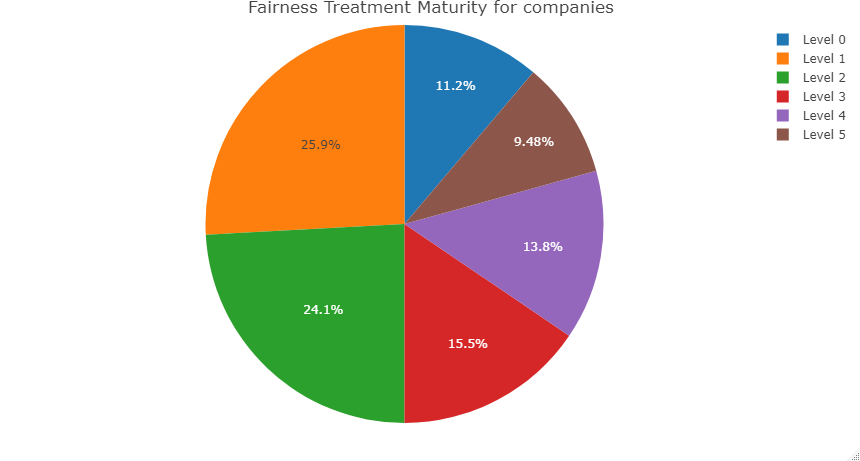
\includegraphics[width=1\textwidth]{figure/Analisi/RQ5/Fairness Treatment Maturity for companies.png}
        \caption{Risultati analitici del Fair Capability Maturity Model}
    \end{figure}
    
    Come risporta la figura 5.23, è facile fornire una risposta preliminare a questo questo di ricerca, il contesto attuale, provando a generalizzare quanto osservabile sulla base del campione, è costituito da circa un \textbf{50\% delle aziende che praticano sviluppo di soluzioni ML-Intensive}, che tratta fairness ai \textbf{livelli 1 e 2}, ovvero, secondo la scala prefissata, trattano le problematiche connesse alla fairness in maniera sporadica o abitudinaria, ma senza l'utilizzo di standard specifici. Interessante anche come dell'altra metà dei partecipanti, soltanto \textbf{l'11,2\% dichiari che la sua azienda non tratti affatto fairness}, infatti \textbf{la fetta restante di partecipanti colloca la propria azienda ai livelli 3, 4 e 5}, quindi dal trattare Fairness in maniera abitudinaria con specifici standard di sviluppo, fino all'applicazione di tecniche di process improoving sugli specifici processi aziendali. 
    
     \begin{figure}[h!]
        \centering
        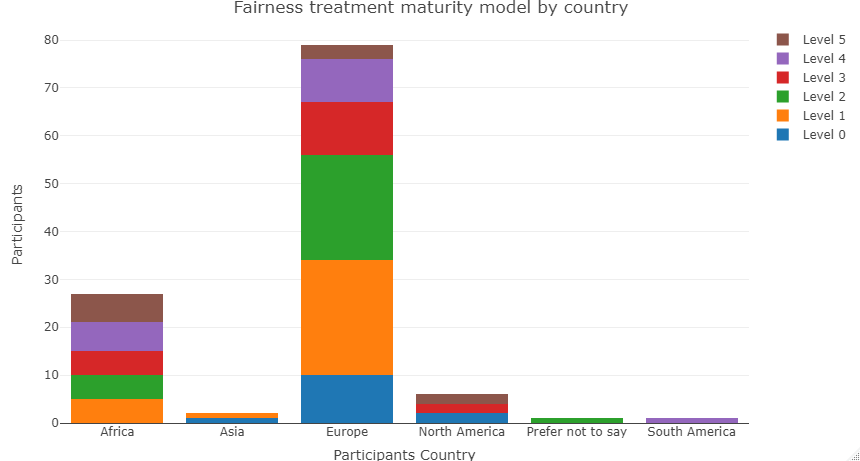
\includegraphics[width=1\textwidth]{figure/Analisi/RQ5/Fairness treatment maturity model by country.png}
        \caption{Risultati analitici del Fair Capability Maturity Model per continente}
    \end{figure}
    
    Spostando l'analisi su un ottica più mirata, come quella continentale - figura 5.24, si nota ancora meglio come ad esempio in Europa (la maggioranza del campione) le aziende pratichino processi atti alla gestione della fairness. Ciò è senz'altro un fattore ampiamente positivo, dato che è facilmente osservabile come le aziende, ad esempio su scala europea, siano disposte a migliorare e ad applicare processi ingegneristici nell'ambito ml intensive, di pari passo all'evoluzione metodologica della ricerca e degli investimenti pubblici \cite{ritson201317}.
    
    \begin{center}
	
        \begin{tcolorbox}[width=\textwidth, colframe=black, colback=Gray]
    			\begin{minipage}{\textwidth}
    				\textit{\faKey  \textbf{ Risultato di ricerca 13}}\\
    		     Il trattamento di fairness è un aspetto ad oggi poco maturo considerando standard e pratiche di sviluppo aziendali, quasi la totalità delle aziende, sulla base del campione, dichiara di trattare l'aspetto etico durante lo sviluppo di soluzioni ML-Intensive, ma la maggior parte lo fa con strategie non mirate all'ottimizzazione dei processi.
    			\end{minipage}
		\end{tcolorbox}
	\end{center}
	
	\begin{center}
	
        \begin{tcolorbox}[width=\textwidth, colframe=black, colback=Gray]
    			\begin{minipage}{\textwidth}
    				\textit{\faKey  \textbf{ Risultato di ricerca 14}}\\
    		     Si evidenzia come altre realtà professionali tendano anche a trattare l'aspetto etico in moduli di machine learning in maniera più oculata, definendo i propri standard di sviluppo, fino all'adottare strategie specifiche di process improoving.
    			\end{minipage}
		\end{tcolorbox}
	\end{center}

    
    
    \section{Discussioni e Implicazioni}
    
    \subsection{Quanto fairness è \emph{matura} nello sviluppo ML aziendale?}
    Partendo dall'analisi dello stato dell'arte, in questo lavoro di tesi si è osservato come effettivamente i ricercatori dell'ambito ingegneristico, evidenzino la necessità di trattare il concetto di software fairness come un vero e proprio aspetto qualitativo \emph{primario} nello sviluppo ML intensive, affinché le elaborazioni dei moduli prodotti e i risultati di predizione degli stessi, siano immuni dal presentare problematiche connesse a vulnerabilità discriminatorie \cite{brun2018software}. Sulla base dei dati raccolti dall'indagine, è senz'altro interessante notare, come la maggior parte delle compagnie coinvolte riconosca l'esistenza di questa problematica ed applichi strategie a riguardo, come osservabile infatti dai risultati del quinto quesito di ricerca, solo una minima parte dei partecipanti dichiara che la propria compagnia non tratta affatto Fairness (11,2 \%) durante i quotidiani processi di sviluppo, mentre, dal lato opposto, oltre il 30 \% dei partecipanti dichiara di 
    applicare Fairness con i dovuti standard propri dell'azienda di appartenenza fino all'applicare strategie specifiche di process improoving nel trattamento di fairness. A conferma di ciò, l'analisi dei dati permette di osservare come tool commerciali per il trattamento di Fairness in un modulo di machine learning esistano e risultano essere estremamente utili nello sviluppo di soluzioni eticamente corrette, in particolare i tools più quotati dagli intervistati sono  Microsoft Fairnlearn, che approccia lo sviluppo fair-critical con casi d'uso reali, e Google What If? che permette proprio di analizzare in maniera qualitativa e quantitativa i livelli di fairness di uno specifico modulo.\\
    
    \begin{center}
	
        \begin{tcolorbox}[width=\textwidth, colframe=black, colback=Gray]
    			\begin{minipage}{\textwidth}
    				\textit{\faSearch  \textbf{ Osservazione 1}}\\
    		     Fairness è percepita sempre di più come un aspetto fondamentale per i moduli ML-Intensive, numerose realtà professionali condividono le necessità evidenziate dal mondo della ricerca e a tal proposito cercano di migliorare i processi di sviluppo con particolare attenzione all'aspetto etico e molto spesso a fare la differenza sono tools o strategie specifiche dei principali vendors conosciuti.
    			\end{minipage}
		\end{tcolorbox}
	\end{center}
    
   \subsection{Quanto fairness è \emph{immatura} nello sviluppo ML aziendale?}
   Concentrandosi invece sui dati rimanenti del quinto punto di ricerca analizzato, va osservato come il 50 \% del campione di analisi, dichiara di trovarsi ai livelli 1 e 2 della scala di maturità formalizzata, quindi è opportuno chiedersi se effettivamente fairness è vista o meno a livello pratico come un aspetto prioritario rispetto altre specifiche non funzionali. Dall'analisi generale dei confronti tra fairness con altri aspetti di qualità in un modulo ML-Intensive si è visto effettivamente come le opinioni raccolte tendano ad essere in ogni caso tendenti al considerare Fairness da lievemente meno rilevante, come per i confronti con aspetti qualitativi appartenenti al modello FURPS+, ad estremamente meno rilevante, come nel caso di specifiche estremamente più tecniche e standardizzate quali Security o Performance del modello. Vero che dall'analisi settoriale è riscontrabile come questa tendenza sia estremamente differente a seconda del dominio specifico, e.g. la differente rilevanza media di Fairness rispetto a Security nei settori di Governance ed Intrattenimento, ma dai dati a disposizione è senz'altro evidente come l'aspetto etico sia ancora poco maturo e standardizzato per essere considerato una vera e propria specifica non funzionale in un modulo di machine learning rispetto a specifiche \emph{storiche} più documentate e standardizzate. Molto probabilmente a tal proposito la chiave di svolta è racchiusa nel supporto che la comunità scientifica può apportare allo stato della pratica, senz'altro incentrando i nuovi studi sulle necessità e percezioni che l'attuale stato della pratica evidenzia, ma anche verificando in maniera sistematica, se quanto già stato fatto fin ora possa essere applicato attivamente in contesti di sviluppo reali.
   
     \begin{center}
	
        \begin{tcolorbox}[width=\textwidth, colframe=black, colback=Gray]
    			\begin{minipage}{\textwidth}
    				\textit{\faCaretSquareORight  \textbf{ Implicazione 1}}\\
    		     Nonostante Fairness sia percepita come una specifica qualitativa di rilevanza dai professionisti, sono molte le aziende che la trattano in maniera poco sistematica o con priorità minore rispetto altre specifiche di qualità più standardizzate. Al fine di invertire definitivamente questa tendenza, nuovi studi di ricerca sono sicuramente necessari e possono fare la differenza.
    			\end{minipage}
		\end{tcolorbox}
	\end{center}
    
    \subsection{Definire e misurare fairness in un caso reale di sviluppo ML}
    Come osservato dalla letteratura, molti sono le definizioni e le metriche formalizzate al fine di trattare fairness durante lo sviluppo ML-Intensive \cite{FairnessDefinitionExplained}. Dai risultati del primo quesito di ricerca, si può notare come gli esperti tendano ad apprezzare in larga misura tutti i gruppi di definizioni proposte, però se si cerca qualche dettaglio in più, è facile osservare come approcci formali basati su similarità matematica, siano leggermente preferiti rispetto ai più formali aspetti basati su puro calcolo probabilistico o su relazioni di dipendenze causali. D'altro canto però, osservando i risultati inerenti il quesito inerente l'applicazione di approcci pratici nel trattamento di fairness, gli stessi intervistati dichiarano di trovarsi più a proprio agio a ragionare intuitivamente sulle dipendenze causali tra feature sensibili e risultati, piuttosto che su aspetti più tecnici, quali possibili attività di tuning dei parametri fair-oriented. A prima vista ciò potrebbe essere quasi un contro senso, ma effettivamente quanto le attuali definizioni basate su dipendenze causali, sono intuibili dai lavoratori se considerate nella loro forma più formale? Quanto i differenti gruppi di definizioni attualmente conosciuti sono applicabili in maniera generale tenendo conto delle svariate esigenze dei domini d'utilizzo? Intersecare ciò che i risultati di analisi ottenuti, si evince anche praticamente l'applicabilità dell'una o l'altra definizione di fairness, oppure l'utilizzo di una o più approcci pratici, dipenda in se per se dal dominio di utilizzo, ciò non solo per l'enorme variabilità di rilevanza riscontrata analizzando a livello settoriale i dati relativi al terzo quesito di ricerca, ma anche perché molti partecipanti facciano presente in maniera esplicita, che oltre agli approcci noti in letteratura, essi stessi facciano uso di tecniche diverse da quelle proposte, ad esempio l'applicazione di strategie empiriche o di indicatori statistici come osservato dall'analisi dei dati. Quindi dove la ricerca può intervenire in tal senso? In definitiva non è probabile che l'una o l'altra strategia sia univocamente condivisibile o applicabile data l'estrema specificità della tematica, ma da un analisi più specifica degli standard di sviluppo effettivamente sarà possibile individuare quali processi formali possano essere o meno applicabili a seconda delle più svariate esigenze di dominio.
    
      \begin{center}
	
        \begin{tcolorbox}[width=\textwidth, colframe=black, colback=Gray]
    			\begin{minipage}{\textwidth}
    				\textit{\faCaretSquareORight  \textbf{ Implicazione 2}}\\
    		     Dall'analisi effettuata è principalmente emerso che l'ampia varietà di metodologie e approcci (più o meno formali) per il trattamento di fairness e la variabile rilevanza delle specifiche etiche rispetto al dominio di utilizzo, sono fattori da cui non si può prescindere. Detto ciò è facilmente intuibile come la specificità del problema è una chiave di lettura essenziale per i futuri studi di ricerca.
    			\end{minipage}
		\end{tcolorbox}
	\end{center}
    
    \subsection{Processi di sviluppo ML Fair-Oriented, una visione a lungo termine}
    
    Constatato che fairness secondo l'attuale stato della pratica continua ad essere un aspetto estremamente dipendete dal dominio applicativo, e che gli studi a riguardo necessitino ancora di essere espansi tenendo conto in primo luogo dei bisogni pratici evidenziati dai professionisti, resta doveroso cercare di capire dove effettivamente la ricerca possa intervenire affinché il trattamento di fairness possa essere sistematizzato al pari di altre specifiche qualitative di un modulo ML-Intensive. È oramai noto alla comunità scientifica, ma anche allo stato della pratica che approcci di sviluppo evolutivo quali il noto standard MLOps, siano una strategia vincente nel trattare e migliorare le specifiche di qualità di un modulo intelligente, soprattutto nel contesto di MLOps, sono nate strategie specifiche che consentono di monitorare i livelli di un particolare aspetto non funzionale, ma ciò è possibile anche nel caso dell'etica? dall'analisi dei dati ricevuti in risposta ai quesiti inerenti le fasi di una canonica pipeline di machine learning e delle figure di rilievo in un team orientato allo sviluppo fair-oriented probabilmente ciò è assolutamente un buon punto su cui riflettere per futuri lavori di ricerca. \\
    
    Partendo proprio dall'analisi delle fasi di una canonica pipeline di machine learning, si è visto come gli esperti del settore propongano come più critico il trattamento di fairness nelle fasi di gestione e manipolazione dei dati di training, validazione del modello oppure nelle statistiche di monitoraggio del modello in esecuzione nel contesto d'utilizzo. Proprio in questo contesto la ricerca offre già numerose soluzioni, basti pensare alle tecniche specifiche di selezione dei dati basate su diversità statistica \cite{moumoulidou2020diverse} oppure alle specifiche tecniche di testing fair-orinted e ribilanciamento del campione \cite{galhotra2017fairness}. Ma quanto queste strategie specifiche, sono conosciute ed applicate dai professionisti? Quanto invece nuove strategie come nuovi modelli di validazione fair-specific sono necessarie per sistematizzare questi processi? tutto questo, quasi sicuramente necessita di ulteriori approfondimenti, e nuovi lavori quali l'analisi di bad \& best practices specifiche per il trattamento di fairness in un modulo ML-Intensive o la ricerca di maggiori cause di discriminazione partendo ad esempio dall'analisi delle principali feature sensibili comuni alla maggior parte dei datasets di addestramento, possono essere senz'altro un buon punto di partenza. In connessione all'applicabilità di strategie, in un qualsiasi processo di sviluppo che si rispetti, va senz'altro definito chi debba assumere l'una o l'altra responsabilità. Dai dati ottenuti si evidenziano due principali osservazioni:
    \begin{itemize}
        \item  Ingegneri del software e data scientist restano a pari merito figure cruciali e di simili rilevanza anche nel trattamento di specifiche problematiche quali i livelli di fairness nei moduli;
        \item La definizione di linee guida di management o il coinvolgimento di esperti specifici per il trattamento di software fairness sono aspetti che maggiormente fanno la differenza.
    \end{itemize}
    
    Ma da queste osservazioni possono anche riscontrarsi nuovi quesiti da porsi ed analizzare, ad esempio:
    
    \begin{itemize}
        \item Quando risulta essere cruciale che ruoli diversi quali data scientist e ingegneri del software lavorino in sinergia se si considera una pipeline di machine learning?
        \item Quali possono essere i punti di partenza per la definizione di standard di management specifici?
        \item Cosa si intende effettivamente per esperti nell'ambito Fairness? Esperti di socio-culturali di etica? Esperti del dominio specifico o quant'altro?
    \end{itemize}
    
    Oltre ciò, anche altri dati possono essere di ispirazione per nuovi studi, non ultimo la minore rilevanza data dai partecipanti ad altri aspetti critici di una pipeline di machine learning come l'ingegnerizzazione dei requisiti o la preparazione del modello. In generale il principale contributo che si evince da questo lavoro di tesi sta proprio nella consapevolezza che l'etica di un modulo di machine learning necessita di maturare ed evolvere in maniera sistematica proprio perché le cause e i fattori che impattano tale tematica oggigiorno sono sempre più evidenti e dai risultati ottenuti è senz'altro intuibile dove sia più utile intervenire in funzione di questi obiettivi.
    
    \begin{center}
	
        \begin{tcolorbox}[width=\textwidth, colframe=black, colback=Gray]
    			\begin{minipage}{\textwidth}
    				\textit{\faSearch  \textbf{ Osservazione 2}}\\
    		     Dai risultati ottenuti, risulta cruciale come i modelli di sviluppo evolutivi (e.g. MLOps), risultano essere particolarmente efficaci nel trattare specifici aspetti di qualità, quali appunto la fairness di un modulo ML-Intensive. Infatti è riscontrabile come per gli esperti del dominio, proprio le caratteristiche etiche del modello evolvono e si raffinano mano mano che il modello stesso matura durante le varie fasi del suo ciclo di vita.
    			\end{minipage}
		\end{tcolorbox}
	\end{center}
	
	 \begin{center}
	
        \begin{tcolorbox}[width=\textwidth, colframe=black, colback=Gray]
    			\begin{minipage}{\textwidth}
    				\textit{\faCaretSquareORight  \textbf{ Implicazione 3}}\\
    		    Ricercare nuove soluzioni per lo sviluppo ML Fair-Oriented o sistematizzare quelle già esistenti, implica un'ottica di analisi che tenga conto della natura evolutiva delle specifiche etiche. Ad esempio gli esperti del settore indicano  fasi specifiche come: Data Preparation o Validazione del modello come cruciali nell'evoluzione di un modulo ML.
    			\end{minipage}
		\end{tcolorbox}
	\end{center}
	
	\begin{center}
	
        \begin{tcolorbox}[width=\textwidth, colframe=black, colback=Gray]
    			\begin{minipage}{\textwidth}
    				\textit{\faCaretSquareORight  \textbf{ Implicazione 4}}\\
    		   Nella definizione di strategie fair-oriented legate allo sviluppo evolutivo dei sistemi ML-Intensive, vanno anche approfonditi aspetti specifici legati alle responsabilità delle singole figure professionali, alcuni punti di studio intuibili dall'indagine sono infatti: la necessità di formalizzare le responsabilità dei manager nel trattamento di fairness, l'overlap di responsabilità tra ingegneri del software e data scientist anche in questo specifico caso, oppure il definire formalmente quali esperti coinvolgere a seconda del problema specifico.
    			\end{minipage}
		\end{tcolorbox}
	\end{center}
	
	\begin{center}
	
        \begin{tcolorbox}[width=\textwidth, colframe=black, colback=Gray]
    			\begin{minipage}{\textwidth}
    				\textit{\faCaretSquareORight  \textbf{ Implicazione 5}}\\
    		    Lavorare con fairness significa anche capire effettivamente come fairness si caratterizza nel dominio specifico, quindi risulta particolarmente importante anche adottare nuove strategie che permettano di mappare definizioni ed approcci sulla base delle specifiche del dominio del problema. In tal senso, sarà senz'altro necessario indagare su nuove metodologie didattiche che approccino la tematica tenendo conto di questa specifica esigenza.
    			\end{minipage}
		\end{tcolorbox}
	\end{center}
\newpage

\chapter{Conclusioni} %\label{1cap:spinta_laterale}
% [titolo ridotto se non ci dovesse stare] {titolo completo}
%


\begin{citazione}
	BREVE SPIEGAZIONE CONTENUTO CAPITOLO
\end{citazione}

\newpage


%\part{Impatto ambientale}

\backmatter
\phantomsection
\chapter{Ringraziamenti}
\markboth{Ringraziamenti}{}
% [titolo ridotto se non ci dovesse stare] {titolo completo}
INSERIRE RINGRAZIAMENTI QUI 
\bibliographystyle{ieeetr}
\bibliography{bibliografia.bib}
\end{document}
